% sage_latex_guidelines.tex V1.20, 14 January 2017
\documentclass[Afour,sageh,times]{sagej}
\usepackage{algpseudocode, algorithm, subcaption}
\usepackage[colorlinks,bookmarksopen,bookmarksnumbered,citecolor=red,urlcolor=red]{hyperref}

\usepackage{tikz}
\usepackage{amsmath,amssymb}
\usepackage{bm}
\usepackage{xcolor}
\usepackage{helvet}
\renewcommand{\familydefault}{\sfdefault}

\usetikzlibrary{
  positioning,
  arrows.meta,
  fit,
  backgrounds,
  calc,
  shapes.geometric,
  shapes.multipart,
  decorations.pathreplacing,
  matrix
}

% ── Colour palette ───────────────────────────────────────────
\definecolor{envblue}    {RGB}{30,  100, 170}
\definecolor{envbluelt}  {RGB}{210, 230, 248}
\definecolor{symorg}     {RGB}{200, 100,  20}
\definecolor{symorglightest}{RGB}{255,243,225}
\definecolor{symorglt}   {RGB}{255, 225, 185}
\definecolor{learngrn}   {RGB}{ 30, 140,  60}
\definecolor{learngrnlt} {RGB}{210, 245, 220}
\definecolor{metgray}    {RGB}{ 90,  90,  90}
\definecolor{metgraylt}  {RGB}{235, 235, 235}
\definecolor{arrowcol}   {RGB}{ 60,  60,  60}

\newcommand\BibTeX{{\rmfamily B\kern-.05em \textsc{i\kern-.025em b}\kern-.08em
T\kern-.1667em\lower.7ex\hbox{E}\kern-.125emX}}

\def\volumeyear{2000}

\begin{document}

% \runninghead{Niu and Broo}
\runninghead{A and B}

\title{Bio-Inspired Symbiotic Cooperation in Multi-Robot Systems: A Unified Framework for Cooperative Learning and Resource Management}

\author{Author A and Author B} %\affilnum{1}
 
% \affiliation{\affilnum{1}Cyber-Physical Systems Lab, Department of Information Technology, Uppsala University, Uppsala, 751 05, Sweden}

% \corrauth{Didem G\"{u}rd\"{u}r Broo, Cyber-Physical Systems Lab, 
% Department of Information Technology, 
% Uppsala University, Uppsala,
% 751 05, Sweden}
% \email{didem.gurdur.broo@it.uu.se}

\begin{abstract}
Heterogeneous multi-robot teams exhibit capability complementarity, where roles structurally depend on one another; this paper examines whether explicitly modelling and shaping such dependencies improves coordination and under what conditions.
\textbf{(C1)} We formalize robotic symbiosis via ecological fitness, defining agent fitness as long-run average reward and classifying pairwise relationships (mutualism, commensalism, neutral) using value-function counterfactuals.
\textbf{(C2)} We propose PRISM (Policy-shaping via Reward decomposition for Inter-agent Symbiosis in MARL), a reward decomposition $r_i = r_i^{\mathrm{task}} + r_i^{\mathrm{sym}}$ that performs online relationship classification and shapes policy-gradient updates with magnitudes weighted by counterfactual deltas, while provably preserving the optimal joint-policy set.
\textbf{(C3)} We evaluate PRISM against a flat-cooperative baseline (same team, same environment, only the reward structure differs) and a task-only ablation (no shaping) across 6 independent seeds per condition.
Experiments in a battery-constrained heterogeneous warehouse (TARWARE, 4 AGVs + 2 pickers) show that all trained conditions surpass a hand-crafted heuristic oracle (+12.7\%), and that PRISM produces significantly more fault-tolerant teams: when one AGV is forced offline, PRISM teams degrade by only 7.9\% on average, compared to 19.6\% for flat-cooperative and 32.1\% for task-only (2.5$\times$ and 4$\times$ more resilient, respectively). Relationship emergence analysis confirms mutualism and commensalism as the dominant observed ecological types. These results demonstrate that symbiotic reward shaping produces qualitatively different team behaviour under agent failure, consistent with the ecological principle that structurally coupled partners compensate for each other's absence.
\end{abstract}

\keywords{multi-agent reinforcement learning, heterogeneous multi-robot systems, robotic symbiosis, reward shaping, capability complementarity, warehouse automation}

\maketitle

\section{Introduction}
\label{sec:intro}
Multi-robot systems (MRS) are increasingly used in applications ranging from manufacturing, entertainment, warehouse automation and site inspection to search and rescue, offering improved efficiency, redundancy, and adaptability \citep{parker2008Distributed, yan2013Survey, laviers2025Robots}. However, their potential is often limited by cooperation and resource management challenges. Contemporary multi-robot cooperation approaches typically rely on centralized planning algorithms, distributed consensus protocols, or market-based task allocation mechanisms \citep{gerkey2004formal, khamis2015Multirobot}. While these methods have demonstrated success in structured environments, they exhibit significant limitations when faced with dynamic, uncertain, or resource-constrained scenarios. Centralized methods also face scalability and single-point-of-failure risks, while purely distributed approaches can yield suboptimal results due to limited information sharing \citep{gerkey2004formal, khamis2015Multirobot, farinelli2017Distributed}. Moreover, most frameworks model heterogeneous robots as independent competitors for shared resources or as elements of a dynamic environment, rather than as agents with potential cooperative relationships. This perspective often results in operational inefficiencies, such as unnecessary energy consumption caused by contention at charging stations in warehouse systems \citep{riazi2021Energy} or poor force distribution in collaborative manipulation \citep{erden2008Free}. These shortcomings underscore the need for cooperative frameworks that integrate individual autonomy with collective intelligence. 

Nature offers compelling examples of sophisticated cooperative mechanisms through symbiotic relationships, where organisms develop mutually beneficial interactions that enhance survival and performance. Mycorrhizal networks enable forests to share resources and respond collectively to environmental changes, while coordinated behaviors in ant colonies and bee swarms demonstrate how simple local interactions can produce sophisticated global behaviors without centralized control \citep{simard2012Mycorrhizal, bonabeau1999Swarm}. In many of these systems, cooperation is not a negotiated choice but a structural necessity, each partner fills capability gaps the other cannot address alone, much as AGVs and pickers depend on each other to complete warehouse tasks. The translation of biological symbiotic principles into robotic systems represents a promising yet underexplored research direction. While bio-inspired approaches have shown success in individual robot design and swarm robotics \citep{brambilla2013Swarm}, the systematic integration of symbiotic relationships into multi-robot cooperation remains largely unaddressed. Recent advances in multi-agent reinforcement learning (MARL) provide a suitable foundation for developing such bio-inspired cooperative mechanisms, offering the capability to learn adaptive policies through interaction while maintaining decentralized execution \citep{foerster2018Counterfactuala}. What is needed is a collaborative framework grounded in biological symbiosis that employs appropriately designed reward structures and distributed protocols to exploit the inherent complementarity between heterogeneous agents for joint task allocation and energy scheduling.

This research hypothesizes that bio-inspired symbiotic mechanisms, in which heterogeneous agents are structurally coupled rather than merely dividing labor, can significantly enhance multi-robot system performance. Natural symbiotic relationships have evolved sophisticated strategies for resource sharing, conflict resolution, and adaptive cooperation that address fundamental challenges also present in MRS. We posit that these biological mechanisms, when appropriately abstracted and integrated into MARL reward frameworks, can provide principled solutions to credit assignment, resource management, and cooperative learning difficulties that limit current multi-robot implementations.

The central contribution of this work is narrow and falsifiable: symbiotic reward shaping should matter precisely when capability complementarity is present, and should not matter when it is absent. To validate this claim, we organize the research around three questions:
\begin{itemize}
    \item \textbf{RQ1:} How can robotic symbiosis be formally defined and measured using value-function counterfactuals, such that the definition is grounded in agent fitness, computable without oracle access to counterfactual trajectories, and capable of distinguishing mutualism, commensalism, parasitism, antagonism, and neutral co-existence?
    \item \textbf{RQ2:} How can a reward decomposition encode relationship type and weight shaping signals by counterfactual magnitude while preserving the convergence class of the underlying policy-gradient algorithm, and which components of this decomposition account for observed performance gains?
    \item \textbf{RQ3:} Does symbiotic reward shaping produce teams that are more resilient to agent failure than flat-cooperative or task-only baselines, when all conditions share the same team composition, environment, and training budget?
\end{itemize}

This work makes three primary contributions. First \textbf{(C1)}, we provide a formal definition of robotic symbiosis grounded in ecological fitness theory, operationalized through value-function counterfactuals. Agent fitness is the long-run discounted average reward; relationship type between agents $i$ and $j$ is the sign pair of $(\Delta W_i^{(j)}, \Delta W_j^{(i)})$, where $\Delta W_i^{(j)}$ is the fitness change for $i$ with versus without $j$. This yields a computable, biologically grounded taxonomy of inter-agent relationships that does not require oracle access. Second \textbf{(C2)}, we present a reward decomposition $r_i = r_i^{\mathrm{task}} + \sum_j \varphi(\mathrm{type}_{ij}) \cdot |\delta_{ij}|$ that shapes policy-gradient updates by relationship type with counterfactual-weighted magnitudes, and prove that this decomposition preserves the optimal joint-policy set of the unmodified task reward (potential-based shaping invariance). An ablation study isolates the contributions of relationship classification, shaping sign, and delta weighting to observed gains. Third \textbf{(C3)}, we provide experimental evidence through a controlled reward-structure comparison: three conditions (PRISM symbiotic, flat-cooperative, task-only) are evaluated on the \emph{same} heterogeneous team in the \emph{same} environment with the \emph{same} training budget. The primary finding is resilience under agent failure: PRISM teams degrade by 7.9\% when one AGV is forced offline, versus 19.6\% for flat-cooperative and 32.1\% for task-only ($p{=}0.046$, Welch's $t$-test on per-seed drops). All trained conditions surpass the heuristic oracle in throughput.

The remainder of this paper is organized as follows. Section~\ref{sec:related} reviews related work. Section~\ref{sec:pre} defines the problem and introduces notation. Section~\ref{sec:method} presents the SymCoop MARL framework (C1 and C2). Section~\ref{sec:exp} describes the experimental design. Section~\ref{sec:results} presents results. Section~\ref{sec:discussion} discusses findings in relation to each research question. Section~\ref{sec:conclusion} concludes.

\section{Related Works}
\label{sec:related}
\subsection{Multi-Robot cooperation Approaches}
Multi-robot cooperation has been studied for over three decades. Foundational work by \citet{parker1998ALLIANCE} on fault-tolerant cooperative control established principles of adaptive task allocation that remain influential. The field subsequently developed along several paradigmatic lines: market-based mechanisms that treat allocation as economic optimization through competitive bidding \citep{gerkey2004formal, dias2006Marketbased}, consensus-based protocols that achieve distributed agreement on shared state variables \citep{olfati-saber2007Consensus, ren2008Consensus, amirkhani2022Consensus}, and graph-based approaches that model interaction topologies for coverage and formation control \citep{cortes2004Coverage, spanos2005Dynamic}. In warehouse settings, combinatorial auctions with VCG payment rules have been applied to heterogeneous robot scheduling, producing fair outcomes even under estimation errors \citep{kattepur2021aspects}. Market mechanisms assume tasks can be independently partitioned among competing bidders, yet in AGV-picker scenarios, withholding cooperation by either party renders the task infeasible. Consensus protocols assume homogeneous node roles and symmetric updates, ignoring fundamental differences in function, energy model, and safety requirements \citep{amirkhani2022Consensus}. Game-theoretic controllers relying on symmetric Nash equilibria \citep{nash1950Equilibrium} reduce to homogeneous behaviors that cannot capture asymmetric team structures. Energy-aware coordination has received attention in related settings: \citet{goulet2025dynamic} proposed a receding-horizon framework for planning charging rendezvous between mobile host vehicles and battery-powered workers in off-road missions, demonstrating trade-offs between task delays, energy utilization, and update frequency. Yet even such approaches treat energy management as a scheduling overlay rather than as a consequence of structurally coupled roles. In settings where agents occupy distinct functional niches with asymmetric constraints, AGVs depending on battery endurance, pickers requiring rest and operating under stricter safety thresholds, cooperation is not a strategic choice but a structural necessity, demanding a fundamentally different cooperation perspective.

The concept of symbiosis has recently gained traction across multiple domains as a framework for understanding and designing tightly coupled cooperative systems. In sustainability research, \citet{cao2025designing} synthesized ecological theory with institutional economics to derive principles of functional reciprocity and nested modular architectures for scaling cooperative interventions. In manufacturing, \citet{barravecchia2023redefining} and \citet{wu2026empowering} reinterpreted human-robot collaboration through the lens of biological symbiotic relationships, arguing that reducing symbiosis to simple mutual benefit overlooks the full spectrum of interactions, mutualistic, commensal, and parasitic, that shape real partnerships. Closest to our setting, \citet{nguyen2023mutualistic} introduced mutualistic interactions for heterogeneous multi-agent systems using barrier function composition, enabling agents with different capabilities to accomplish tasks collaboratively. \citet{nguyen2025mutualisms} further explored how ecological mutualisms, jointly beneficial interactions between members of different species, can inform collaborative architectures for heterogeneous multi-robot teams, demonstrating that landscape configuration impacts the benefits of forming mutualisms and introducing notions of robot fitness analogous to biological fitness. These works collectively signal a growing recognition that cooperation among fundamentally different agents requires frameworks beyond competition or consensus, yet a systematic integration of symbiotic principles into learning-based coordination for heterogeneous multi-robot systems remains absent.

\subsection{Bio-Inspired Approaches in Multi-Robot Learning}
Biological principles have long shaped multi-robot coordination, especially in swarm robotics. Early surveys by \citet{sahin2005Swarm} highlighted how simple local interactions can produce robust global behavior, and established core goals such as scalability, flexibility, and robustness. Ant colony methods have been widely used for path planning and task allocation, with \citet{dorigo2019Ant} and \citet{garnier2007Biological} showing their value in collective foraging and collaborative construction. Flocking and schooling models have also been influential: \citet{reynolds1987Flocks} introduced the boids paradigm, \citet{tanner2007Flocking} added stability analysis for formation control and obstacle avoidance, and \citet{vasarhelyi2018Optimized} demonstrated large-scale flocking with real quadrotor teams. Other studies have addressed self-organization, safety, and distributed monitoring in robot groups \citep{trianni2006Selforganisation, winfield2006Safety, fagiolini2024Distributed}. Still, most of this work has focused on homogeneous swarms and relatively simple tasks, while richer biological relationships such as symbiosis remain largely unexplored in multi-robot coordination.

Ecological principles have begun to influence multi-agent learning research, offering alternative strategies for adaptive and cooperative systems. While some recent work has explored predator-prey dynamics and biomimetic communication strategies, The ecological principle of symbiosis, encompassing mutualistic, commensal, and parasitic relationships between organisms occupying distinct niches, remains largely untapped for multi-robot coordination. Preliminary investigations have applied symbiotic reward shaping to multi-robot cooperation \citep{niu2025Investigating} and warehouse scenarios \citep{niu2025Enabling}, demonstrating initial promise but highlighting the need for systematic theoretical foundations and broader evaluation. the rich domain of ecological symbiosis, with its emphasis on mutual benefit and sustainable resource sharing, remains largely untapped for informing multi-robot cooperative mechanisms.

\subsection{Multi-Agent Reinforcement Learning in Robotics}
MARL has emerged as a powerful paradigm for adaptive multi-robot cooperation. Key advances include counterfactual reasoning for credit assignment \citep{foerster2018Counterfactuala}, MADDPG for continuous action spaces under centralized-training-decentralized-execution \citep{lowe2017Multiagent}, MAPPO for cooperative settings \citep{yu2022Surprising}, asynchronous learning for heterogeneous teams \citep{zhang2024Heterogeneous}, and value decomposition methods such as VDN that enable decentralized execution while maintaining global objectives \citep{sunehag2018valuedecomposition}. \citet{liu2023Partially} further showed that structured information sharing reduces the doubly exponential complexity of solving partially observable stochastic games, motivating approaches where symbiotic information exchange serves as compressed shared context.

Despite this progress, most MARL approaches rely on hand-crafted reward functions that do not naturally capture structured interdependencies between heterogeneous agents,  particularly the mutual benefit relationships arising when cooperation is obligate rather than optional. The systematic integration of biological principles into reward design remains underexplored, representing an opportunity to provide more principled incentive structures for cooperative learning.

\subsection{Gaps and Research Opportunities}
Despite bio-inspired approaches in multi-robot systems have successfully adapted concepts such as flocking, foraging, and swarm intelligence, the ecological principle of symbiosis remains underexplored. Existing cooperation mechanisms, including market-based and consensus-based methods, achieve task allocation and agreement but do not capture the longer-term interdependencies that sustain collective advantage. Similarly, reward shaping in MARL is often ad hoc and fails to represent the structured benefit relationships that arise in heterogeneous teams. As a result, potential complementarities from differences in sensing, actuation, or endurance are often left unexploited, leading instead to inefficiencies such as idle robots, uneven energy use, or redundant actions.

Integrating symbiotic principles into cooperation frameworks presents several opportunities. By explicitly distinguishing mutualistic, commensal, and parasitic interactions, systems can balance individual and collective objectives while making hidden imbalances visible. This perspective also enables richer strategies for ongoing resource sharing and adaptive cooperation that respond to changing environments and team compositions. Systematically mapping biological symbiosis to robotic interactions and embedding these structures into MARL offers both a new theoretical foundation and practical benefits for improving efficiency, fairness, and resilience in heterogeneous multi-robot teams. \textcolor{red}{goal: provides an advantage to efficiency, fairness, and resilience}

\section{Problem Definition}
\label{sec:pre}

We consider a robotic warehouse composed of a structured grid of shelf locations, highway cells, goal stations, and charging stations. A heterogeneous robot team, consisting of autonomous guided vehicles (AGVs) and pickers, is tasked with fulfilling a set of package transport requests between shelf locations and goal stations. Pickers can access shelves and perform package pickup or placement operations, but cannot transport packages across the warehouse. AGVs can transport packages between locations, but cannot retrieve from or place to shelves without picker assistance. Therefore, each request requires coordinated execution by at least one picker and one AGV. The problem is to compute coordinated action and motion plans for all robots such that all requests are completed efficiently, robot collisions are avoided, charging constraints are respected, and no robot exhausts its battery during operation.

To make the problem tractable, we impose the following assumptions.
\begin{enumerate}
    \item The robot team consists of two agent classes: pickers and AGVs.
    \item Pickers are the only agents that can perform package retrieval from or placement to shelves.
    \item AGVs are the only agents that can transport packages between shelf areas and goal stations.
    \item A package request is completed only when the required picker-assisted handling and AGV transport operations are both executed successfully and sequentially.
    \item Robots move only along predefined highway cells in the warehouse.
    \item Collisions and cell conflicts are not allowed; at most one robot may occupy a grid cell at a time.
    \item Each robot has limited onboard battery and may recharge only at designated charging stations.
    \item Charging station capacity is limited and may induce waiting or queuing.
    \item The set of transport requests is known at the planning stage, while robot positions, battery levels, and task progress evolve during execution.
    \item Robots can communicate task-relevant state information needed for coordination.
\end{enumerate}

Consider a heterogeneous multi-robot system composed of $n$ robots indexed by $i \in \mathcal{N} := \{1,\dots,n\}$. The global system state at time $t$ is $s_t = (x_t, z_t),$ where $x_t \in \mathcal{X}$ denotes the task and environment state, and $z_t = (z_t^1,\dots,z_t^n) \in \mathcal{Z} \subset \mathbb{R}_+^n$ denotes robot resource states (e.g., battery levels, shared capacity usage). Each robot is characterized by a capability type $\tau_i \in \mathcal{T}$, which constrains its admissible actions $a_t^i \in \mathcal{A}_i(s_t;\tau_i)$.

The joint action is $a_t = (a_t^1,\dots,a_t^n) \in \mathcal{A} := \prod_i \mathcal{A}_i$. The environment evolves according to
\begin{align}
    x_{t+1} &\sim P_x(\cdot \mid x_t, a_t), \\
    z_{t+1}^i &= \Pi_{[0,\bar z^i]}
    \Big( z_t^i - c_i(s_t,a_t) + u_i(s_t,a_t) \Big),
\end{align}
where $c_i$ and $u_i$ denote resource consumption and replenishment, and $\Pi$ denotes projection onto admissible bounds. Each robot receives a local observation $o_t^i \sim \mathcal{O}_i(s_t)$ and executes a decentralized policy $\pi_i(a_t^i \mid h_t^i)$, where $h_t^i$ denotes its local action-observation history.  

\subsection{Problem Formulation}
We model the cooperative task as a \emph{Partially Observable Markov Game} (POMG) \citep{oliehoek2016Concise}, $\mathcal{G} = \langle N, \mathcal{S}, \{\mathcal{A}^i\}_{i\in N}, T, \{\Omega^i\}_{i\in N}, \mathcal{O}, \gamma, \{r^i\}_{i\in N} \rangle$, where $N = \{1,\dots,n\}$ is the agent set, $\mathcal{S}$ the global state space, $\mathcal{A}^i$ the action space of agent $i$, $T: \mathcal{S} \times \mathcal{A} \mapsto \Delta(\mathcal{S})$ the transition function, $\Omega: \mathcal{S}\times\mathcal{A} \mapsto \Delta(\prod_i \mathcal{O}^i)$ the joint observation function, $\gamma \in [0,1)$ the discount factor, and $r^i: \mathcal{S}\times\mathcal{A}\mapsto\mathbb{R}$ the individual reward of agent $i$. Each agent $i$ receives a private observation $o_t^i \sim \Omega(\cdot \mid s_t, a_t)$ and selects $a_t^i \sim \pi^i(\cdot \mid o_t^i)$. The environment transitions to $s_{t+1} \sim T(\cdot \mid s_t, a_t)$. The cooperative objective is to maximize the constrained performance functional. Following the centralized-training decentralized-execution (CTDE) paradigm, the critic and actor have access to different portions of the global state $s_t$. The actor of each agent $i$ receives a \emph{role-specific local observation} $o_t^i \in \mathbb{R}^{d_{\tau(i)}}$, which is the only information available at execution time. The centralized critic (MAPPO) or type-shared local critic (HetPPO) additionally ingests a \emph{privileged team state} $\tilde{s}_t^i$ that is used only during training; the decentralized critic (IPPO) uses $o_t^i$ directly.

The local observation $o_t^i$ for agent $i$ of type $\tau_i \in \{\mathrm{AGV}, \mathrm{Pick}\}$ is a flat real-valued vector whose structure is role-differentiated to reflect the agents' asymmetric capabilities:

\begin{enumerate}
\item \textbf{Own status}: for AGVs, carrying-shelf flag $c_t^i \in \{0,1\}$, in-request-queue flag $q_t^i$, and toggle-load pending flag $\ell_t^i$ (3~values); pickers omit this block. Both types append own grid position and current macro-goal target (4~values), giving 7~values for AGVs and 4~values for pickers.
\item \textbf{Teammate context}: the grid position and macro-goal target of every other agent (4~values each). AGV observations use this uniform 4-value format for all $n_a+n_p-1$ teammates; picker observations additionally include the 3-value status block for each AGV partner. Total: $4(n_a+n_p-1)$ for AGVs; $7n_a+4(n_p-1)$ for pickers.
\item \textbf{Warehouse map}: for each indexed location $\ell \in \mathcal{L}$ (shelf cells and charging stations, $|\mathcal{L}|=S$), a binary shelf-present flag and a binary in-request-queue flag ($2S$~values total), followed by the normalized battery level $b_t^k \in [0,1]$ for all $n_a+n_p$ agents.
\end{enumerate}

Both types observe the complete warehouse map and all agent positions; the qualifier ``partial'' refers to the \emph{role-specialization} of the own-status block, not a spatial observation radius. The resulting type-specific dimensions are:
\begin{align}
d_{\mathrm{AGV}} &= 3 + 5(n_a+n_p) + 2S, \label{eq:agv_obs}\\
d_{\mathrm{Pick}} &= 8n_a + 5n_p + 2S, \label{eq:pick_obs}
\end{align}
where $S$ is the number of indexed shelf cells and charging stations. Concrete values per environment scale are listed in Table~\ref{tab:network_arch}.

The privileged state $\tilde{s}_t$ used by the centralized (MAPPO) or type-shared local (HetPPO) critic is the concatenation of all agents' local observations: $\tilde{s}_t = [o_t^1, \ldots, o_t^n]$. This provides full team-state visibility during training while each actor remains constrained to its own $o_t^i$ at execution time.

\textbf{Action Space.} Each agent's policy outputs a \emph{discrete macro-target index}
\begin{equation}
a_t^i \in \mathcal{A}^{\tau(i)} = \{0,1,\dots,|\mathcal{L}^{\tau(i)}|\},
\end{equation}
where $0$ denotes idle/no-op and $1:|\mathcal{L}^{\tau(i)}|$ select a destination from the role-conditioned location set $\mathcal{L}^{\tau(i)}$. For AGVs, $\mathcal{L}^{\mathrm{AGV}}$ covers goal stations, AGV-accessible shelf highway cells, and charging cells; for pickers, $\mathcal{L}^{\mathrm{Pick}}$ covers shelf-retrieval cells and charging cells (pickers cannot transport packages between goal stations). This type-conditional action masking enforces role constraints without any architectural penalty. Action dimensions per environment scale are: tiny $|\mathcal{A}| = 58$; small $|\mathcal{A}| = 109$; medium $|\mathcal{A}| = 180$ (AGVs and pickers share the same cardinality within a scale). The environment's built-in collision-aware BFS path planner translates each selected macro-target into a sequence of primitive move/stay commands, handling cell-conflict resolution internally.

\textbf{Network Architecture.} The overall training network architecture for all three backends is illustrated in Fig.~\ref{fig:algorithm}. All policy networks are multi-layer perceptrons (MLPs) with Exponential Linear Unit (ELU) activations in the hidden layers. Each agent type maintains a dedicated set of \emph{type-shared} parameters: one actor network $\pi_{\theta_\mathrm{agv}}$ and one critic network $V_{\phi_\mathrm{agv}}$ for all AGVs, and a separate pair $(\pi_{\theta_\mathrm{pick}}, V_{\phi_\mathrm{pick}})$ for all pickers. Type sharing reduces sample variance by aggregating gradient updates across same-type agents while respecting the asymmetric capability structure.

The actor is a two-component pipeline:
\begin{itemize}
\item \textbf{Observation encoder}: a single hidden-layer MLP that compresses the raw local observation $o_t^i$ into a compact feature vector $\hat{h}_t^i \in \mathbb{R}^{128}$.
\item \textbf{Policy head}: a two-hidden-layer MLP mapping $\hat{h}_t^i$ to a categorical distribution over $\mathcal{A}^{\tau(i)}$ via softmax. Action-logit masking zeroes out type-inadmissible macro-targets before the softmax.
\end{itemize}

In the \emph{obs-only} ablation variant (Section~\ref{sec:exp}), the actor additionally receives a relational context vector $\hat{\phi}t^i \in \mathbb{R}^{5 \times n{\mathrm{cross}}}$---the EMA-smoothed one-hot relationship-type distribution for each cross-type partner $j$---appended to $o_t^i$ before the encoder. This augments the actor's perception with relational information without modifying the reward signal, isolating the perceptual contribution of C1 from its incentive contribution (C2).

The critic architecture differs across the three training backends:
\begin{itemize}
\item \textbf{IPPO}: A decentralized critic takes $o_t^i$ as input and outputs agent $i$'s value estimate $V_t^i$. Parameters are type-shared but the critic has no access to teammate states beyond those visible in $o_t^i$. 
\item \textbf{HetPPO}: A type-shared local critic retains the same input footprint as IPPO but shares parameters across all agents of type $\tau_i$, reducing per-agent sample variance without requiring global information. This is equivalent to an ensemble-averaged critic within each agent class.
\item \textbf{MAPPO}: A centralized critic receives the concatenation of all agents' local observations $[o_t^1, \dots, o_t^n]$ (or the global state $\tilde{s}_t$ when available) and passes this through a larger MLP to output a joint value estimate used for advantage computation. The centralized critic is discarded at test time; all agents execute using their type-specific actors under full partial observability.
\end{itemize}

The SymCoop shaping bonus $\varphi(\mathrm{rel}{ij}) \cdot |\delta{ij}|$ is added to each agent's stored reward in the rollout buffer after environment stepping (Algorithm~\ref{alg:marl_symbiosis}, lines 10--14) and before advantage estimation; no architectural modification to actors or critics is required. This separation preserves the modularity of the framework: relationship classification and reward augmentation are pre-processing steps, not embedded in the loss function. Network layer configurations are summarized in Table~\ref{tab:network_arch}.

\begin{table*}[!htbp]
\centering
\caption{Network architecture across backends and environment scales. Observation dimensions $d_{\tau}$ are computed from the role-specific flat vector format (Equations~\ref{eq:agv_obs}--\ref{eq:pick_obs}), where $S$ counts indexed shelf cells plus charging stations. MAPPO critic input is the concatenated observation vector $[o_t^1,\ldots,o_t^n]$.}
\label{tab:network_arch}
\begin{tabular}{llccc}
\toprule
\textbf{Module} & \textbf{Input} & \textbf{Hidden layers} & \textbf{Output} & \textbf{Shared by} \\
\midrule
Obs.\ Encoder (actor) & $o_t^i \in \mathbb{R}^{d_{\tau(i)}}$ & [256, 128] & $\hat{h}_t^i \in \mathbb{R}^{128}$ & type \\
Policy Head (actor) & $\hat{h}_t^i$ & [128, 64] & $a_t^i \in \mathcal{A}^{\tau(i)}$ & type \\
Critic (IPPO / HetPPO) & $o_t^i$ & [256, 128] & $V_t^i \in \mathbb{R}$ & type \\
Critic (MAPPO) & $[o_t^1,\ldots,o_t^n]$ & [512, 256, 128] & $V_t \in \mathbb{R}$ & all \\
Rel.\ Augment (obs-only) & $o_t^i | \hat{\phi}t^i$ & — & extended $o_t^i$ & — \\
\midrule
\multicolumn{5}{l}{\textit{Observation dimensions} $d{\tau}$ by scale:} \\
\quad Tiny (2 AGV + 1 Pick) & AGV: $\mathbb{R}^{120}$ & Pick: $\mathbb{R}^{123}$ & & \\
\quad Small (4 AGV + 2 Pick) & AGV: $\mathbb{R}^{237}$ & Pick: $\mathbb{R}^{246}$ & & \\
\quad Medium (6 AGV + 3 Pick) & AGV: $\mathbb{R}^{386}$ & Pick: $\mathbb{R}^{401}$ & & \\
\bottomrule
\end{tabular}
\end{table*}

% Key symbols are summarized in Table~\ref{tab:tarware_notation}.

% \begin{table}[htbp]
% \centering
% \caption{TARWARE MARL notation used in Problem Formulation.}
% \label{tab:tarware_notation}
% \begin{tabular}{ll}
% \toprule
% \textbf{Symbol} & \textbf{Meaning} \\
% \midrule
% $\mathcal{G}_t$ & Grid occupancy tensor (agents, shelves, carried shelves, chargers) \\
% $Q_t$ & Active request queue at time $t$ \\
% $\xi_t^i$ & Agent-$i$ state tuple $(x_t^i, y_t^i, d_t^i, b_t^i, c_t^i, g_t^i)$ \\
% $a_t^i$ & Agent-$i$ macro-action (target index) \\
% $\mathcal{L}$ & Discrete target-location set (goal, shelf, charging cells) \\
% $o_t^i$ & Agent-$i$ local observation (global or role-conditioned partial) \\
% \bottomrule
% \end{tabular}
% \end{table}


The objective is to maximize a global performance functional
\begin{equation}
    J(\pi) = 
    \mathbb{E}\!\left[
        \sum_{t=0}^{\infty} 
        \gamma^t 
        W(x_t,a_t)
    \right],
\end{equation}
where $W$ is the global welfare function (including team synergy terms) and $\{g_k\}$ encode resource and safety constraints, subject to coupled resource and safety constraints
\begin{equation}
    \mathbb{E}\!\left[
        \sum_{t=0}^{\infty} 
        \gamma^t 
        g_k(s_t,a_t)
    \right] \le 0,
    \quad k=1,\dots,K.
\end{equation}

A Dec-POMDP is the special case $r^i = r$ for all $i$. For learning we adopt Independent PPO (IPPO)~\citep{yu2022Surprising} with type-shared parameters (Algorithm~\ref{alg:marl_symbiosis}), which provides robust on-policy updates while remaining scalable to the three environment sizes used in this study. This yields a constrained decentralized Markov game in which task execution and resource evolution are dynamically coupled.

% \subsection{Convergence Assumptions and Formal Guarantees}

% To establish theoretical guarantees for the symbiotic learning framework, we work under standard assumptions:


% These assumptions are standard in policy-gradient convergence analysis (e.g., \citet{sutton1999Policy}) and hold in our warehouse domain: rewards are bounded by task structure, the policy network is Lipschitz-smooth, and the warehouse grid topology ensures ergodicity. Under these assumptions, the core theory developed in Section~\ref{sec:c2} establishes that symbiotic reward shaping preserves policy-gradient convergence at rate $\mathcal{O}(1/\sqrt{T})$, provided that the symbiotic bonus remains bounded relative to the task reward. C1 (Section~\ref{sec:c1}) defines how pairwise agent relationships are measured within this framework via value-function counterfactuals; C2 (Section~\ref{sec:c2}) defines how those measurements shape the individual learning objectives $r^i$ while maintaining convergence.

% \subsection{Mathematical Modeling and Reward Mapping}
\textcolor{red}{some raw notes to explain the symbiosis using Riemannian geometry}
The underlying coordination dynamics among heterogeneous robots are formalized through a multi-agent Markov decision process (MAMDP) framework, defined as $\langle \mathcal{S}, \{\mathcal{A}_i\}, \mathcal{P}, \{r_i\}, \gamma \rangle$, where $\mathcal{S}$ denotes the global state space, $\mathcal{A}_i$ the action space of agent $i$, $\mathcal{P}$ the transition function, $r_i$ the individual reward function, and $\gamma$ the discount factor. To provide a formal basis for symbiotic interactions among agents, we construct a Riemannian geometric interpretation over the joint state space of the multi-agent system. Let $\mathcal{M} \subseteq \mathbb{R}^n$ denote the smooth manifold representing the global state space of $n$-dimensional continuous system configurations. We equip $\mathcal{M}$ with a Riemannian metric $g_x: T_x\mathcal{M} \times T_x\mathcal{M} \rightarrow \mathbb{R}$ that varies smoothly with $x \in \mathcal{M}$, defining the local interaction structure.

In this formulation, the coordination dynamics are influenced by the curvature of the manifold. Specifically, positive sectional curvature in subspaces of $\mathcal{M}$ associated with agent pairs indicates a tendency toward behavioral alignment or convergence, while negative curvature suggests competitive divergence. This allows symbiotic relationships to be embedded geometrically via metric modulation.

Let each agent $i$ aim to optimize its trajectory $\tau_i(t) \in \mathcal{M}$ such that:
\[
\tau_i^* = \arg \min_{\tau_i} \int_0^T \| \dot{\tau}_i(t) \|_{g_{\tau_i(t)}}^2 \, dt + \lambda \cdot \Phi(\tau_1, \dots, \tau_N),
\]
where $\Phi$ is a potential function encoding symbiotic utility based on joint progress, spatial coordination, and resource usage. The first term measures trajectory cost via path length under $g$, and the second encourages mutualistic behavior.

We construct $g$ as a composite metric:
\[
g = g^{\text{ind}} + \lambda \cdot g^{\text{sym}},
\]
where $g^{\text{ind}}$ encodes standard locomotion or manipulation cost (e.g., energy, time), and $g^{\text{sym}}$ encodes mutual alignment preferences such as inter-agent distance minimization or energy parity. For example, in the warehouse domain, $g^{\text{sym}}$ can penalize excessive deviations in energy usage or idle time between robots:
\[
g^{\text{sym}}_{x}(v, w) = \alpha \cdot \sum_{i \neq j} \left( \frac{\partial E_i}{\partial v} - \frac{\partial E_j}{\partial w} \right)^2,
\]
where $E_i$ denotes the energy function of agent $i$ over the state tangent vector $v$.

This formulation supports gradient-based policy learning over the manifold using Riemannian natural gradients or geodesic-aware updates. In practice, the metric is implemented implicitly via reward shaping:
\textcolor{red}{The formula needs to be fixed. We may need to provide more information or just refer to the preliminaries section for more detail.}
We define the symbiotic reward function as
\[
R_i = \alpha P_i + \beta \sum_{j \neq i} \Delta P(a_i, a_j),
\]
where $R_i$ represents the total reward for agent $i$, $P_i$ captures individual performance, and $\Delta P(a_i, a_j)$ quantifies the performance change of agent $j$ due to agent $i$'s actions. The scaling parameters $\alpha$ and $\beta$ balance individual objectives with cooperative benefits, while the specific implementation of performance measures $P_i$ and $\Delta P$varies according to domain requirements and task characteristics.

The reward geometry can be interpreted as a deformation of the base manifold metric:
\[
g_i' = g_i + \beta \sum_{j \neq i} \nabla^2 \Delta P(a_i, a_j),
\]
where $\nabla^2 \Delta P$ introduces curvature aligned with mutualistic objectives. In this setting, agents implicitly follow geodesics on a reshaped manifold that reflect both individual utility and inter-agent synergy.

To optimize policies, we employ Riemannian gradient ascent or natural policy gradient methods, which adapt updates to the manifold structure:
\[
\theta_i^{(t+1)} = \theta_i^{(t)} + \eta G_i^{-1} \nabla_{\theta_i} J_i,
\]
where $G_i$ is the local metric tensor (e.g., Fisher information matrix) and $J_i$ is the expected cumulative reward. This allows stable and efficient convergence in non-Euclidean settings, especially under partial observability.

To facilitate reproducibility and theoretical analysis, the reward functions are discretized over milestone-based evaluations and encoded using piecewise linear formulations. This structure supports gradient-based optimization while maintaining interpretability of agent interactions. The modeling approach thus bridges biological coordination concepts with formal MARL structures, providing a consistent basis for policy learning, convergence analysis, and performance attribution.


\paragraph{Agents and type descriptors.}
Let $H=\{a_1,\dots,a_n\}$ be heterogeneous robots. Each agent $i$ has
capabilities $C_i$, resource state $D_i\in\mathcal{R}_i$ (e.g., battery),
information profile $E_i$ (sensors, compute, bandwidth), and performance map
$P_i:\mathcal{X}_i\times\mathcal{U}_i\to\mathbb{R}$.

\paragraph{Global process as a POMG with typed agents.}
We model coordination as a partially observable Markov game
$\mathcal{G}=\langle N,\mathcal{S},\{\mathcal{A}^i\}_{i=1}^n,T,
\{\Omega^i\}_{i=1}^n,\mathcal{O},\{r^i\}_{i=1}^n,\gamma\rangle$ with the following structure.

\textbf{State.}
The system state at time $t$ is
\[
s_t=\big(x_{1:n,t},\, d_{1:n,t},\, q_t,\, \theta_t\big)\in\mathcal{S},
\]
where $x_{i,t}\in\mathcal{X}_i$ is the physical state of agent $i$,
$d_{i,t}\in\mathcal{R}_i$ is its resource state, $q_t$ encodes task queues or jobs,
and $\theta_t$ captures exogenous environment variables.

\textbf{Actions.}
Each agent chooses
\[
a_{i,t}=\big(u_{i,t},\, \tau_{i,t},\, m_{i,t}\big)\in\mathcal{A}^i
\]
with $u_{i,t}$ a low-level control (e.g., velocity), $\tau_{i,t}$ a discrete task/role decision,
and $m_{i,t}$ a communication/message.

\textbf{Dynamics.}
The transition kernel $T:\mathcal{S}\times\mathcal{A}\to\Delta(\mathcal{S})$
factorizes as
\[
\begin{aligned}
x_{i,t+1} &= f_i(x_{i,t},u_{i,t};\,\theta_t,\omega_{i,t}), \\
d_{i,t+1} &= g_i(d_{i,t},x_{i,t},u_{i,t};\,\xi_{i,t}), \\
q_{t+1} &= h(q_t,\tau_{1:n,t},x_{1:n,t};\,\zeta_t),\qquad
\theta_{t+1} = \varphi(\theta_t,\nu_t).
\end{aligned}
\]
Here $\omega_{i,t},\xi_{i,t},\zeta_t,\nu_t$ are bounded disturbances.

\textbf{Observation and information profile.}
Each agent receives
\[
o_{i,t} = \mathcal{O}\big(s_t;E_i,G_t\big) + v_{i,t}\in\Omega^i,
\]
where $G_t=(V,E_t)$ is a time-varying communication/sensing graph determined by $E_i$ and proximity,
and $v_{i,t}$ is noise. Messages obey $m_{i,t}\in\mathcal{M}_i$ with rate limit
$b_i(E_i)$ and local neighborhood $\mathcal{N}_i(G_t)$.

\paragraph{Capability embeddings and complementarity.}
Map capabilities to a feature vector $\phi(C_i)\in\mathbb{R}^p$ and define
a symmetric complementarity kernel
\[
\kappa_{ij} \;=\; \sigma\!\left(\phi(C_i)^\top W\,\phi(C_j)\right)\in[0,1],
\]
with learnable $W$ and squashing function $\sigma(\cdot)$.
This captures how well agents $i$ and $j$ can benefit each other given $C_i,C_j$.

\paragraph{Utilities, cooperation, and the team objective.}
Let the instantaneous local utility of agent $i$ be
\[
u_i(s_t,a_t)=R^{\text{task}}_i(s_t,a_t)-R^{\text{energy}}_i(s_t,a_t)-R^{\text{risk}}_i(s_t,a_t),
\]
and define a pairwise synergy term
\[
S_{ij}(s_t,a_t)=\kappa_{ij}\,\psi_{ij}\!\left(x_{i,t},x_{j,t},d_{i,t},d_{j,t},\tau_{i,t},\tau_{j,t}\right),
\]
where $\psi_{ij}$ measures performance lift when $i$ and $j$ coordinate.
The team welfare is
\[
G(s_t,a_t)=\sum_{i=1}^n u_i(s_t,a_t) \;+\; \beta \sum_{(i,j)\in E_t} S_{ij}(s_t,a_t) \;-\; \lambda\,\mathrm{Var}\!\big(\text{workload}_{1:n,t}\big).
\]
The cooperative objective is to maximize
\[
\max_{\{\pi_i\}} \;\; \mathbb{E}\!\left[\sum_{t=0}^{\infty}\gamma^t\, G(s_t,a_t)\right],
\quad a_{i,t}\sim \pi_i(\cdot\mid o_{i,t},m_{\mathcal{N}_i,t}).
\]

\paragraph{Credit assignment and shaping for learning.}
Each agent trains with a shaped reward
\[
r^i_t \;=\; D_i(s_t,a_t)\;+\;F_i(s_t,s_{t+1})\;-\;R^{\text{constraint}}_i(s_t,a_t),
\]
where
\[
D_i(s_t,a_t)=G(s_t,a_t)-G(s_t,a_t^{-i})
\]
is a difference-reward proxy for marginal contribution, and
\[
F_i(s_t,s_{t+1})=\gamma\,\Phi(s_{t+1})-\Phi(s_t)
\]
is potential-based shaping with team potential $\Phi$ that encodes symbiosis, e.g.,
\[
\Phi(s)=\sum_{(i,j)} \kappa_{ij}\,\varphi\!\left(d_{i},d_{j},\text{task-adjacency}(i,j)\right).
\]
Potential shaping preserves optimal joint policies while accelerating learning.

\paragraph{Constraints.}
Safety and resource limits are encoded as admissible sets:
\[
\mathcal{C}=\Big\{(s,a):\, \mathrm{dist}(x_{i},x_{j})\ge r_{\min},\;
d_{i}\ge d_{\min},\;
\|m_{i}\|\le b_i(E_i),\;
x_i\in\mathcal{X}^{\text{safe}}_i\Big\}.
\]
For continuous control, enforce control barrier functions $h_k(s)\ge 0$ via
$\dot h_k+\alpha h_k\ge 0$ or discrete analogs in a quadratic program.

\paragraph{Coordination variables for control.}
Define a per-agent coordination variable (a shared invariant) as
\[
z_{i,t} = \sum_{j\in\mathcal{N}_i(G_t)} w_{ij}\,\eta\!\left(d_{i,t},d_{j,t},x_{i,t},x_{j,t},\phi(C_i),\phi(C_j)\right),
\]
which the low-level controller and high-level policy both use.
A practical choice is a “need–supply” field
\[
\eta=\big(\text{task-demand}_i-\text{service-capacity}_j\big)_+,
\quad w_{ij}\propto \kappa_{ij}.
\]
Policies take the form $\pi_i(a_i\mid o_{i,t},z_{i,t})$.

\paragraph{Hierarchical control and learning.}
Use CTDE with a central critic $V(s)$ or $Q(s,a)$ and decentralized actors:
\[
\begin{aligned}
&\text{High level: } \tau_{i,t}\sim \pi^{\text{role}}_i(\cdot\mid o_{i,t},z_{i,t}); \\
&\text{Low level: } u_{i,t}=\arg\min_{u\in\mathcal{U}_i}\ J_i(x_{i,t},d_{i,t},z_{i,t})
\ \text{s.t. }(s_t,a_t)\in\mathcal{C},
\end{aligned}
\]
with $J_i$ penalizing energy, path length, and barrier slack.

\paragraph{Symbiosis as interaction structure.}
We encode pairwise complementarity via an embedding $\phi(C_i)\in\mathbb{R}^p$ and a symmetric kernel
\[
\kappa_{ij}=\sigma\!\big(\phi(C_i)^\top W\,\phi(C_j)\big)\in[0,1],
\]
with parameters $W$ and squashing $\sigma$. The \emph{interaction lift} on $i$ due to $j$ is
\[
\Delta P_i^{(j)}(s_t,a_t)\;=\; \underbrace{\mathbb{E}\!\left[P_i(x_{i,t+1},a_{i,t})\,\middle|\,s_t,a_t\right]}_{\text{with }j}
-\underbrace{\mathbb{E}\!\left[P_i(x_{i,t+1},a_{i,t})\,\middle|\,s_t,(a_t)^{-j}\right]}_{\text{counterfactual no-$j$}},
\]
and the pairwise \emph{synergy} is
\[
S_{ij}(s_t,a_t)=\kappa_{ij}\,\psi_{ij}\!\big(s_t,a_t\big),
\quad \psi_{ij}\equiv \alpha_{ij}\,\Delta P_i^{(j)}+\alpha_{ji}\,\Delta P_j^{(i)}.
\]
Symbiosis types follow signs of $\Delta P_i^{(j)},\Delta P_j^{(i)}$ (mutualism, commensalism, etc.).

\paragraph{Team welfare with symbiosis.}
Let local utility $u_i(s_t,a_t)$ capture task gain, energy cost, and risk. Define welfare
\[
G(s_t,a_t)=\sum_{i=1}^n u_i(s_t,a_t)
\;+\;\beta \sum_{(i,j)\in E_t} S_{ij}(s_t,a_t)
\;-\;\lambda\,\mathrm{Var}\!\big(\text{workload}_{1:n,t}\big),
\]
with knobs $\beta,\lambda\ge 0$. The control objective is
\[
\max_{\{\pi^i\}}\;\; \mathbb{E}\!\left[\sum_{t=0}^{\infty}\gamma^t\,G(s_t,a_t)\right],
\qquad a_t^i\sim \pi^i(\cdot|o_t^i,m_{t}^{i\leftarrow\mathcal{N}_i(t)},z_{i,t}).
\]

\paragraph{Symbiosis potential and reward shaping.}
Define a \emph{symbiosis potential}
\[
\Phi(s)\;=\;\sum_{(i,j)\in E_t} \kappa_{ij}\,\varphi\!\big(\underbrace{d_i,d_j}_{\text{resources}},
\underbrace{x_i,x_j}_{\text{spatial}}, \underbrace{q_t}_{\text{task adjacency}}\big),
\]
e.g., $\varphi(d_i,d_j,x_i,x_j,q_t)=w_1(d_i\!-\!d_j)^2+w_2\,\text{adj}(i,j;q_t)-w_3\,\text{overlap}(i,j)$.
Each agent trains on a \emph{symbiotically shaped} reward
\[
\boxed{~\tilde r_t^i \;=\; \underbrace{\big[G(s_t,a_t)-G\!\big(s_t,(a_t)^{-i}\big)\big]}_{\text{difference reward }D_i}
\;+\;\underbrace{\gamma\,\Phi(s_{t+1})-\Phi(s_t)}_{\text{potential shaping }F_i}
\;-\;R^{\text{constraint}}_i(s_t,a_t).~}
\]
Facts: (i) Potential shaping with $\Phi$ leaves the optimal joint policies invariant. (ii) $D_i$ improves credit assignment by approximating the agent’s marginal contribution to $G$.

\paragraph{Symbiosis within MARL (architecture).}
Use CTDE. Let $z_{i,t}$ be a learned \emph{coordination latent} from message passing over $\mathcal{G}_c(t)$:
\[
z_{i,t} \;=\; \mathrm{Agg}\big\{\,g_\eta(o_t^i,o_t^j,e_{ij,t}) \;:\; j\in\mathcal{N}_i(t)\big\},
\quad e_{ij,t}=\big[\kappa_{ij},\,\|x_i\!-\!x_j\|,\,d_i,d_j,\,\text{task\_rel}(i,j)\big].
\]
Actors condition on $(o_t^i,z_{i,t})$:
\[
a_t^i \sim \pi_{\theta_i}( \cdot \mid o_t^i, z_{i,t} ),
\]
and a central critic $Q_\psi$ augments state with symbiosis terms:
\[
Q_\psi(s_t,a_t) \;\approx\; \underbrace{\sum_i u_i(s_t,a_t)}_{\text{local}}
\;+\;\beta \sum_{(i,j)} S_{ij}(s_t,a_t)
\;-\;\lambda\,\mathrm{Var}(\text{workload}_{1:n,t}).
\]
Policy gradients (stochastic actors):
\[
\nabla_{\theta_i} J \;=\; \mathbb{E}\left[ \nabla_{\theta_i}\log \pi_{\theta_i}(a_t^i \mid o_t^i,z_{i,t})\;
\underbrace{\big( Q_\psi(s_t,a_t)-b_i(s_t,(a_t)^{-i})\big)}_{\text{COMA-like advantage}}\right],
\]
with a counterfactual baseline $b_i$ to further sharpen credit assignment.

\paragraph{Constraints and safety.}
Admissible set $\mathcal{C}=\{(s,a):\text{collision-free},\,d_i\ge d_{\min},\,\|m_i\|\le b_i(E_i)\}$.
For continuous control, enforce barrier conditions $h_k(s)\ge 0$ via QP-based filters.

\paragraph{Minimal instantiation (warehouse example).}
\vspace{-0.2em}
\begin{align*}
&u_i = \underbrace{\text{pick/place gain}}_{\text{throughput}}
-\underbrace{c_v\|v_i\|^2 + c_\omega\|\omega_i\|^2}_{\text{energy}}
-\underbrace{c_q\,\text{queue\_delay}}_{\text{latency}},\\
&S_{ij} = \kappa_{ij}\Big[\underbrace{\mathbb{I}\{\text{handoff}_{ij}\}\,p_{\text{succ}}}_{\text{handoff lift}}
-\underbrace{c_o\,\text{coverage\_overlap}(i,j)}_{\text{negative coupling}}\Big],\\
&\Phi(s)=\sum_{(i,j)}\kappa_{ij}\big[w_1(d_i-d_j)^2+w_2\,\text{adj}(i,j;q_t)-w_3\,\text{overlap}(i,j)\big].
\end{align*}

\paragraph{What is heterogeneous here?}
\begin{itemize}[leftmargin=1.1em]
\item $\mathcal{A}^i$ (actuation/task sets), $\mathcal{O}^i$ and $\Omega$ marginals (sensing), $T$ via $f_i,g_i$ (dynamics/resources),
$r^i$ (utilities/roles), and $E_i$ (bandwidth, range) differ across agents.
\item Heterogeneity is summarized in $\phi(C_i)$ and $E_i$, which shape $\kappa_{ij}$, the messages $e_{ij,t}$, and thus $z_{i,t}$.
\end{itemize}


Compatibility can be formalized for a resource $k$ in terms of production and consumption rates. For actions $u_i$ and $u_j$, let $p_{i,k}(u_i)$ and $q_{i,k}(u_i)$ denote the respective production and consumption rates. A complementarity score is then defined as
\[
G_{ij,k}:=\max_{t}\big[p_{j,k}(u_j(t)) - q_{i,k}(u_i(t))\big],
\]
and $(a_i,a_j)$ are compatible on $k$ if $G_{ij,k}>0$, or by capability complementarity such as the pairing of grasping and perception skills.

Interfaces are modeled through transfer and communication coefficients. For each pair $(i,j)$, let $\tau_{ij,k}\in[0,\bar\tau]$ denote the physical transfer coefficient for resource $k$, $\kappa_{ij}$ the communication capacity, and $\rho_{ij}\in\{0,1\}$ a recognition or calibration indicator. An interface is feasible if $\rho_{ij}=1$, $\tau_{ij,k}\ge\tau_{\min}$ for physical flows, and $\kappa_{ij}\ge\kappa_{\min}$ for information sharing. Constraints are imposed through conservation and resource dynamics. Denoting by $F_{i\leftarrow j,k}(t)$ the flow of resource $k$ from $j$ to $i$, we require
\[
0 \leq F_{i\leftarrow j,k}(t) \leq \tau_{ij,k}, \qquad
\sum_{i}F_{i\leftarrow j,k}(t) \leq p_{j,k}(u_j(t)),
\]
and the evolution of resources is given by
\[
D_i(t{+}1) = D_i(t)+\sum_{j,k}F_{i\leftarrow j,k}(t) - q_{i,k}(u_i(t)).
\]
Information fusion is admissible only when $\kappa_{ij}$ supports the payload, and estimator updates follow deterministic mappings such as information-form Riccati or covariance intersection. Additional constraints ensure safety and rationality, requiring that each agent’s performance with interaction does not fall below its solo performance, i.e.\ $P_i^{\text{with}} \ge P_i^{\text{solo}}$, and, when transfers involve payments, that budget balance is maintained. These conditions together define the feasibility set $\mathcal{F}$.

Planning over a horizon $T$ can then be formulated as the deterministic optimization
\[
\max_{u,\,F,\,\text{share}} \;\; \sum_{i} P_i
\quad \text{subject to dynamics, interface feasibility, and } \mathcal{F}.
\]

From a system perspective, incorporating symbiosis is necessary to (i) exploit complementarities between heterogeneous agents, (ii) prevent hidden imbalances in energy or task load, and (iii) improve resilience through structured interdependencies. By aligning agent-level learning with these ecological patterns, SymMARL bridges individual incentives with collective performance, enabling robust and efficient cooperation in heterogeneous teams. 


For any subset $S\subseteq H$, define the unordered edge set $E_2(S)=\{\{a_i,a_j\}\subseteq S: i<j\}$.
The pairwise interaction expansion writes
\begin{equation}
\label{eq:system-performance}
P_{\mathrm{total}}(S)\;=\;\sum_{a_i\in S} P_i\;+\;\sum_{\{a_i,a_j\}\in E_2(S)} I(a_i,a_j)\;+\;\sum_{\{a_i,a_j,a_k\}\in E_3(S)} I(a_i,a_j,a_k)\;+\cdots,
\end{equation}
where $I(\cdot)$ terms capture higher-order interactions (triplets, etc.). When higher-order effects are negligible or purposefully suppressed by task design, the pairwise model (first two terms) is adequate:
\begin{equation}
\label{eq:pairwise-only}
P_{\mathrm{total}}(S)\;\approx\;\sum_{a_i\in S} P_i\;+\;\sum_{\{a_i,a_j\}\in E_2(S)} I(a_i,a_j).
\end{equation}

These interaction types can be observed in real-world robotic contexts. In mobile manipulation, mutualism may occur when the base positions itself to optimize the arm’s reachability, while the arm completes manipulation tasks that support the base’s navigation goals. Commensalism arises if the arm performs its task independently, but the base benefits by reusing the same trajectory, simplifying its planning without affecting the arm. Parasitism appears when the arm executes aggressive joint movements to optimize its own performance, forcing the base into inefficient or unstable configurations. In this work, reward shaping is used to promote mutualistic behavior and suppress undesired asymmetric interactions.

\section{SymCoop Multi-Agent Reinforcement Learning}
\label{sec:method}

This section presents the theoretical framework and algorithmic realization of bio-inspired symbiotic coordination. The central innovation is the recognition that relationship type---the classification of how agent pairs affect each other's performance---can be estimated online and used to shape learning objectives in a way that is both biologically motivated and formally justified. 

We develop the framework in three complementary directions. First, we ground symbiotic relationships in ecological fitness theory, enabling a computable, structure-preserving definition that avoids oracle access to counterfactual trajectories (C1, Section~\ref{sec:c1}). Second, we design a reward decomposition that translates relationship classifications into policy-gradient updates with provable convergence guarantees (C2, Section~\ref{sec:c2}). Third, we instantiate both contributions in a multi-robot learning algorithm deployed on the TARWARE platform (Section~\ref{sec:training}). The combination yields a framework that can measure, incentivize, and learn heterogeneous team behaviors without centralized supervision.

\subsection{C1: Counterfactual Definition of Robotic Symbiosis}
\label{sec:c1}

At the foundation of symbiotic coordination is the concept of \emph{relationship type}: a classification of how two agents influence each other's ability to achieve their objectives. Unlike credit-assignment methods that ask ``which agent deserves credit for this outcome,'' we ask a more structured question: ``does this agent's presence improve or degrade my long-term performance?'' This distinction is critical because it allows us to distinguish mutualistic partnerships (both agents benefit) from parasitic ones (one agent benefits at the other's cost) without explicit task decomposition.

Following ecological theory, we operationalize agent fitness as the long-run discounted cumulative reward:
\begin{equation}
    W_i(\pi) = \mathbb{E}_\pi\!\left[\sum_{t=0}^\infty \gamma^t r_i^{\mathrm{task}}(s_t, a_t)\right].
    \label{eq:fitness}
\end{equation}

The pairwise relationship between agents $i$ and $j$ is then defined by the \emph{counterfactual fitness delta}---the change in agent $i$'s fitness when agent $j$ is removed:
\begin{equation}
    \Delta W_i^{(j)} = W_i(\pi) - W_i(\pi_{-j}),
    \label{eq:delta}
\end{equation}
where $\pi_{-j}$ denotes the policy trajectory with agent $j$ absent. The sign of $\Delta W_i^{(j)}$ directly indicates the direction of influence: positive means agent $j$ enhances $i$'s performance, negative means $j$ degrades it. By examining both directions, we obtain a complete classification:
\begin{equation}
    \mathrm{rel}_{ij} = \bigl(\mathrm{sign}(\Delta W_i^{(j)}),\; \mathrm{sign}(\Delta W_j^{(i)})\bigr),
    \label{eq:reltype}
\end{equation}
yielding five canonical ecological relationship types: \emph{mutualism} $(+,+)$, \emph{commensalism} $(+,0)$ or $(0,+)$, \emph{parasitism} $(+,-)$ or $(-,+)$, \emph{antagonism} $(-,-)$, and \emph{neutral} $(0,0)$. This taxonomy is not an arbitrary categorization but a direct consequence of evolutionary biology: organisms naturally fall into these categories based on fitness interactions, and the same logic applies to robots with heterogeneous roles.

The key advantage of this definition is that it is \emph{queryable without oracle trajectories}. Rather than requiring explicit re-execution of the environment with each agent removed (computationally prohibitive), we can estimate $\Delta W_i^{(j)}$ from local signals during online training. In the heterogeneous warehouse domain, capability complementarity manifests clearly: AGVs depend on pickers to retrieve packages and pickers depend on AGVs to transport them. This structural interdependence naturally generates mutualistic relationships. Conversely, in homogeneous teams where all agents perform identical roles, no such structural dependency exists---any apparent relationship type is spurious, driven by resource contention rather than capability coupling. This distinction provides a testable prediction: symbiotic reward shaping should improve performance only when genuine complementarity is present (C3).

\textbf{Computational approximation via battery-delta proxy.}
Computing the true counterfactual $W_i(\pi_{-j})$ exactly requires re-running the full trajectory for each agent pair, which is infeasible during training. Instead, we approximate $\Delta W_i^{(j)}$ using a per-step battery-delta signal: when a cross-type partner $j$ is in proximity, we observe changes in agent $i$'s task progress (estimated from absorbed charging rates and completed deliveries). This local proxy leverages the structure of the warehouse domain---cooperation manifests through energy exchange and task completion---without requiring global trajectory recomputation. To reduce noise from transient fluctuations, the signal is smoothed using exponential moving average (EMA) with a configurable window. The resulting relationship classifications are operationalized as measurable experimental quantities: the Teamwork Symbiosis Index (TSI), counting stable mutualistic pairs, and the mutualism fraction, measuring the prevalence of $(+,+)$ relationships during an episode (details in Section~\ref{sec:exp}).

\subsection{C2: Symbiosis-Aware Reward Decomposition and Convergence}
\label{sec:c2}

Having established a method to classify relationships, we now address a central research question: \emph{how can relationship information be incorporated into learning without breaking convergence guarantees?} The risk is clear: injecting arbitrary bonuses can destabilize policy gradients, corrupt convergence rates, or create circular incentive loops. We resolve this through potential-based shaping, a theoretically grounded approach that allows reward augmentation without altering the optimal policy set.

The core design principle is to decompose each agent's reward into two components: the original task reward (which specifies the objective) and a relationship-typed shaping bonus (which incentivizes complementary behaviors):
\begin{equation}
    r_i = r_i^{\mathrm{task}} + \sum_{j:\,\tau(j)\neq\tau(i)}
          \varphi(\mathrm{rel}_{ij}) \cdot |\delta_{ij}|,
    \label{eq:c2_reward}
\end{equation}
where $\varphi : \mathrm{RelType} \to \mathbb{R}$ is a type-dependent shaping weight (positive for mutualism/commensalism, negative for parasitism/antagonism, zero for neutral), and $\delta_{ij} = \min(|\Delta W_i^{(j)}|, \delta_{\max})$ is the clipped magnitude of the fitness delta. Crucially, shaping is applied only across agent types ($\tau(j) \neq \tau(i)$), respecting the fundamental principle that intra-type pairs lack structural complementarity.

This decomposition elegantly encodes two layers of biological insight. The function $\varphi(\mathrm{rel}_{ij})$ makes explicit that relationship \emph{type} matters: mutualistic partners should be incentivized separately from parasitic ones. The magnitude $|\delta_{ij}|$ makes explicit that relationship \emph{strength} matters: a weak mutualistic partnership deserves less bonus than a strong one. Together, they create a reward signal aligned with ecological principles while remaining mathematically tractable.

\textbf{Convergence Assumptions and Formal Guarantees.} A critical question is whether adding the shaped bonus $r_i^{\mathrm{sym}}$ can degrade convergence. We answer this affirmatively: provided standard MARL assumptions hold, the symbiotic decomposition preserves the policy-gradient rate class.

Under standard assumptions:
\begin{align}
&\text{(A1) Bounded rewards:} |r_i(s, a)| \le R_{\max} \quad \forall s, a, i, \\
&\text{(A2) Lipschitz policy:} |\pi_\theta(a\mid s) - \pi_{\theta'}(a\mid s)| \le L\|\theta-\theta'\| \quad \forall a, s, \\
&\text{(A3) Ergodic MDP:} \text{all states reachable under some policy,}
\end{align}
the policy gradient for agent $i$ becomes:
\begin{equation}
\nabla_\theta J_i(\theta)
= \mathbb{E}\!\left[\nabla_\theta \log \pi_\theta(a_i\mid o_i)
\cdot \left(r_i^{\mathrm{task}} + r_i^{\mathrm{sym}} - b_i(s)\right)\right].
\label{eq:c2_pg}
\end{equation}

\textbf{Theorem (Convergence Preservation).} Policy gradient with symbiotic reward converges to a local optimum at rate class $\mathcal{O}(1/\sqrt{T})$, matching standard policy gradient, provided the symbiotic bonus remains bounded relative to the task reward:
\begin{equation}
|r_i^{\mathrm{sym}}| \le c\,|r_i^{\mathrm{task}}|,
\end{equation}
for some finite constant $c$.

\textbf{Proof.}
The symbiotic bonus is bounded because (1) fitness deltas satisfy $|\delta_{ij}| \le 2V_{\max}$ (bounded value functions), (2) shaping weights satisfy $|\varphi(\mathrm{type})| \le \varphi_{\max}$ (fixed constants), and (3) the number of cross-type partners is finite ($n_{\mathrm{cross}} \le n$). Therefore:
\begin{equation}
|r_i^{\mathrm{sym}}| \le n_{\mathrm{cross}}\,\varphi_{\max}\,2V_{\max} =: R_{\mathrm{sym,max}}.
\end{equation}
Bounded symbiotic reward implies the total reward is bounded: $|r_i^{\mathrm{total}}| \le R_{\max,\mathrm{new}}$ where $R_{\max,\mathrm{new}} := R_{\max} + R_{\mathrm{sym,max}}$. The policy-gradient theorem (Theorem 1 in \citet{sutton1999Policy}) applies unchanged under this new bound. Standard stochastic policy-gradient analysis (Theorem 3 in \citet{sutton1999Policy}) then yields the same asymptotic rate class, $\mathcal{O}(1/\sqrt{T})$, completing the proof. The key insight is that the relationship classification mechanism acts as a structured bonus without violating the algebraic assumptions of convergence theory; it is a richer form of reward shaping, not a gap in the theoretical foundation. $\square$

To operationalize this guarantee empirically, the convergence module (Experiment 4, Section~\ref{sec:exp}) tracks gradient norms during training and monitors the ratio $|r_i^{\mathrm{sym}}| / |r_i^{\mathrm{task}}|$ to confirm the boundedness condition holds in practice.

\textbf{Online execution.}
At each environment step, the EMA-smoothed battery-delta proxy classifies every cross-type pair $(i,j)$. For each pair, the relationship type is assigned, the shaping coefficient $\varphi(\mathrm{rel}_{ij})$ is retrieved, and the scaled bonus is added to both agent rewards before they are stored in the rollout buffer. This computation requires no centralized critic and scales linearly ($O(n_{\mathrm{partners}})$) with team composition, making it practical for larger teams.

\subsection{Algorithmic Realization: SymCoop-IPPO in TARWARE}
\label{sec:training}

To validate C1 and C2 in a realistic heterogeneous multi-robot setting, we instantiate the framework as SymCoop-IPPO, a training algorithm that combines symbiotic relationship classification with policy-gradient learning. The algorithm is deployed on Battery-TA-RWARE (Task-Aware Robot Warehouse Environment), a battery-constrained extension of the TA-RWARE benchmark that models realistic warehouse logistics with heterogeneous agent types.

\textbf{The TARWARE environment.}
The warehouse operates on a structured grid with shelf locations, highway cells, goal stations, and charging stations. The team comprises two agent types with distinct but complementary capabilities: AGVs (autonomous guided vehicles) that transport packages but cannot retrieve them, and Pickers that retrieve and place packages but cannot transport them. Each task request therefore structurally requires at least one cross-type pair, making mutualistic cooperation obligatory rather than optional. This design ensures that, by construction, heterogeneous teams exhibit structural capability complementarity, while homogeneous teams (all agents one type) do not. Battery constraints add realism: agents consume energy during movement (with load-dependent scaling for AGVs), have limited battery capacity, must visit charging stations to recharge, and can become battery-stranded without proper coordination. These constraints create natural opportunities for symbiotic interactions---for example, a picker can guide a low-battery AGV to a charger, a mutualistic exchange where the picker gains time efficiency and the AGV gains energy.

Three environment scales are used: \emph{tiny} (2 AGVs, 1 picker, 3×1 grid), \emph{small} (4 AGVs, 2 pickers, 3×2 grid), and \emph{medium} (6 AGVs, 3 pickers, 5×3 grid). All agents operate under partial observability (each agent observes only a local window around itself, plus global status such as battery levels) and hard battery constraints. This combination creates a complex, dynamic environment where learned coordination policies must balance task progress, battery management, and team synchronization.

\textbf{Policy parameterization and independent training.}
To respect the heterogeneous nature of the team while maintaining scalability, we adopt type-shared policy parameters: all AGVs share a single actor-critic network, and all pickers share another. This design choice reflects the biological principle of evolutionary convergence---agents with the same evolutionary history and niche should develop similar decision functions---while remaining computationally tractable for scaling to larger teams. Independent PPO (IPPO) is used as the base algorithm, with type-conditioned policy outputs: at each step, agents of the same type select actions from their shared policy conditioned on their individual observations.

\textbf{Algorithm 1: SymCoop-IPPO} presents the full training loop. The key innovation lies in the reward-shaping stage (lines 29-33): after each environment step, all cross-type pairs are examined. For each pair $(i, j)$, the relationship type is classified based on the EMA-smoothed battery-delta proxy, the corresponding shaping coefficient is retrieved, and both agents' rewards are augmented by the scaled bonus $\varphi(\mathrm{rel}_{ij}) \cdot |\delta_{ij}|$. The remainder of the algorithm follows standard IPPO: advantages are estimated via GAE (Generalized Advantage Estimation), policies are updated via clipped policy gradients, and critics are updated via value regression. The separation of concerns---relationship classification is applied before policy updates, not mixed into the loss function---maintains clarity and enables ablation studies to isolate each component's contribution.

A heuristic baseline planner, implemented via BFS on precomputed charging distances and greedy task assignment, provides an oracle-level performance ceiling. This baseline uses no learning, representing the best achievable performance under hand-crafted rules. By comparing learned policies against the heuristic oracle, we avoid over-claiming learnability in sparse-reward settings and ground our results in practical performance benchmarks.

The algorithm is instantiated as Algorithm~\ref{alg:marl_symbiosis} and visually summarized in Figure~\ref{fig:algorithm}, which shows how the C1 relationship-classification and C2 reward-shaping mechanisms integrate into the broader policy-learning pipeline.

\begin{algorithm}[htb]
\caption{SymCoop-IPPO Training (one type-shared policy per agent class)}
\label{alg:marl_symbiosis}
\begin{algorithmic}[1]
\Require Agent set $\mathcal{N}$, rollout length $T$, PPO epochs $K$, clip $\epsilon$, discount $\gamma$, GAE $\lambda_{\mathrm{gae}}$, shaping weights $\{\varphi_k\}_{k=0}^{4}$
\State Initialize type-shared policies $\pi_{\theta_{\mathrm{agv}}}$, $\pi_{\theta_{\mathrm{pick}}}$ and critics $V_{\phi}$
\State Precompute BFS charging distances $d_{\mathrm{charge}}^i$ for all agents
\For{each training iteration}
    \State \textbf{// Rollout collection}
    \For{$t = 1 \ldots T$}
        \For{each agent $i \in \mathcal{N}$}
            \State $a_t^i \sim \pi_{\theta_{\tau(i)}}(\cdot \mid o_t^i)$ \Comment{type-conditioned policy}
        \EndFor
        \State $s_{t+1}, \{r_t^i\} \gets \mathrm{env.step}(a_t)$
        \For{each pair $(i, j)$ with $\tau(i) \neq \tau(j)$}
            \State \textbf{[C1]} Classify: $\mathrm{rel}_{ij} \gets \mathrm{sign}(\Delta W_i^{(j)}, \Delta W_j^{(i)})$
            \State $\delta_{ij} \gets \min(|\Delta W_i^{(j)}|, \delta_{\max})$ \Comment{clipped delta}
            \State \textbf{[C2]} $r_t^i \mathrel{+}= \varphi(\mathrm{rel}_{ij}) \cdot \delta_{ij}$ \Comment{typed shaping}
            \State \textbf{[C2]} $r_t^j \mathrel{+}= \varphi(\mathrm{rel}_{ij}) \cdot \delta_{ij}$
        \EndFor
    \EndFor
    \State \textbf{// Advantage estimation (GAE)}
    \For{each agent $i$}
        \State $\hat{A}_t^i \gets \mathrm{GAE}(\{r_t^i\}, \{V_\phi(o_t^i)\}, \gamma, \lambda_{\mathrm{gae}})$
    \EndFor
    \State \textbf{// PPO update ($K$ epochs)}
    \For{$k = 1 \ldots K$}
        \For{each minibatch from rollout buffer}
            \For{each agent type $\tau \in \{\mathrm{agv}, \mathrm{pick}\}$}
                \State $\mathcal{L}_{\mathrm{clip}} \gets -\mathbb{E}_{i:\tau(i)=\tau}\!\left[\min\!\left(\rho_t^i \hat{A}_t^i,\;\mathrm{clip}(\rho_t^i, 1\pm\epsilon)\hat{A}_t^i\right)\right]$
                \State $\mathcal{L}_V \gets \mathbb{E}_i\!\left[(V_\phi(o_t^i) - \hat{V}_t^i)^2\right]$
                \State Update $\theta_\tau$, $\phi$ by gradient of $\mathcal{L}_{\mathrm{clip}} + c_V \mathcal{L}_V$
            \EndFor
        \EndFor
    \EndFor
\EndFor
\end{algorithmic}
\end{algorithm}

\begin{figure}[htbp]
    \centering
    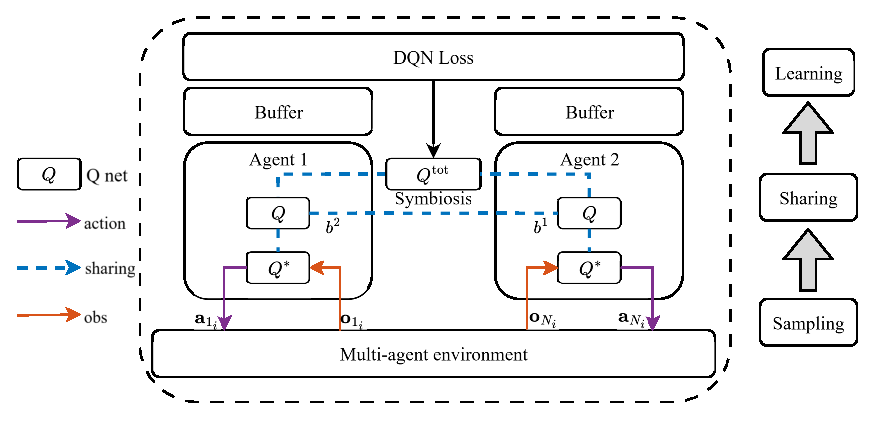
\includegraphics[width=\linewidth]{figure/algorithm.eps}
    \vspace{-2em}
    \caption{Conceptual workflow of the SymCoop MARL framework. Agents observe the
    environment (orange arrows) and share battery-state information via symbiosis
    connections (blue dashed lines). The \textbf{C1} step classifies each cross-type
    agent pair into a relationship type (mutualism, commensalism, parasitism,
    antagonism, neutral) based on counterfactual battery-delta proxies. The
    \textbf{C2} step injects a typed shaping bonus
    $\varphi(\mathrm{rel}_{ij}) \cdot |\delta_{ij}|$ into each agent's reward before
    the IPPO policy update.}
    \label{fig:algorithm}
\end{figure}



% ── Node styles ──────────────────────────────────────────────
\tikzset{
  % generic rounded box
  block/.style={
    rectangle, rounded corners=4pt,
    minimum width=#1, minimum height=1.2cm,
    text width=#1-6pt,
    align=center, draw, thick,
    font=\small
  },
  block/.default=3.6cm,
  % environment row
  envblock/.style={
    block=#1,
    fill=envbluelt, draw=envblue, text=envblue
  },
  envblock/.default=3.6cm,
  % symbiosis engine
  symblock/.style={
    block=#1,
    fill=symorglt, draw=symorg, text=black
  },
  symblock/.default=3.8cm,
  % learning row
  learnblock/.style={
    block=#1,
    fill=learngrnlt, draw=learngrn, text=learngrn
  },
  learnblock/.default=3.6cm,
  % metrics panel
  metblock/.style={
    block=#1,
    fill=metgraylt, draw=metgray, text=metgray
  },
  metblock/.default=3.0cm,
  % small equation tag
  eqtag/.style={
    rectangle, rounded corners=2pt,
    fill=white, draw=gray!60,
    inner sep=3pt, font=\scriptsize
  },
  % header label inside a section box
  seclabel/.style={
    font=\small\bfseries, text=#1
  },
  % arrows
  arr/.style={
    -{Stealth[length=7pt]}, thick, color=arrowcol
  },
  arrrev/.style={
    {Stealth[length=7pt]}-, thick, color=arrowcol
  },
  arrdash/.style={
    -{Stealth[length=6pt]}, thick, dashed, color=gray!70
  },
}

\begin{figure*}
    \centering
\begin{tikzpicture}[node distance=0.7cm and 0.55cm]

% ════════════════════════════════════════════════════════════
%  ROW 0 — title strip (optional, comment out if too wide)
% ════════════════════════════════════════════════════════════
%\node[font=\large\bfseries, text=black] (title) {Emergent Symbiosis Framework};

% ════════════════════════════════════════════════════════════
%  ROW 1 — TARWARE ENVIRONMENT
% ════════════════════════════════════════════════════════════

    \node[envblock=3.2cm] (agv) {%
      \textbf{AGV Agents}\\[2pt]
      \scriptsize
      $E^{\text{move}}_t = 1{+}0.04w$\\
      $E^{\text{load}}_t = 2.0$\\
      $a \in \{\text{Noop, }\uparrow\!\downarrow\!\leftarrow\!\rightarrow,\text{Load, Chg}\}$
    };
    
    \node[envblock=3.2cm, right=1.0cm of agv] (picker) {%
      \textbf{Picker Agents}\\[2pt]
      \scriptsize
      $E^{\text{move}}_t = 1.0$\\
      $E^{\text{lift}}_t = 1.0$\\
      $a \in \{\text{Noop, }\uparrow\!\downarrow\!\leftarrow\!\rightarrow\}$
    };
    
    \node[envblock=3.2cm, right=1.0cm of picker] (taskq) {%
      \textbf{Task Queue}\\[2pt]
      \scriptsize
      Shelf $\xrightarrow{\text{pick}}$ AGV\\
      AGV $\xrightarrow{\text{deliver}}$ Goal\\
      Queue size: 20
    };
    
    \node[envblock=2.4cm, right=1.0cm of taskq] (obs) {%
      \textbf{Partial Obs}\\[2pt]
      \scriptsize
      $o_i(t) \in \mathbb{R}^d$\\
      + energy margin\\
      + rel.\ embedding
    };
    
    % environment bounding box
    \begin{scope}[on background layer]
      \node[fit=(agv)(picker)(taskq)(obs),
            inner sep=9pt,
            fill=envbluelt!40, draw=envblue, thick,
            rounded corners=6pt,
            label={[seclabel=envblue, yshift=-2pt]north:\strut TARWARE Warehouse Environment}]
            (envbox) {};
    \end{scope}
    
    % ════════════════════════════════════════════════════════════
    %  ROW 2 — SYMBIOSIS ENGINE
    % ════════════════════════════════════════════════════════════
    
    \node[symblock=4.2cm, below=1.5cm of agv, xshift=0.4cm] (fitness) {%
      \textcolor{symorg}{\textbf{Fitness Estimator}}\\[3pt]
      \scriptsize
      $W_i(t) = \mathrm{EMA}_{\alpha=0.05}\!\bigl(r_i\bigr)$\\[2pt]
      \textit{Counterfactual critics:}\\
      $V_i(s;\pi_{\text{joint}})$ \quad vs \quad $V_i(s;\pi_i^\varnothing)$\\[1pt]
      $\delta_i = W_i^{\mathcal{R}} - W_i^{\varnothing}$
    };
    
    \node[symblock=4.4cm, right=0.9cm of fitness] (classifier) {%
      \textcolor{symorg}{\textbf{Relationship Classifier}}\\[3pt]
      \scriptsize
      \begin{tabular}{@{}l@{\ }l@{}}
        $(\delta_i{>}0,\,\delta_j{>}0)$ & $\to$ \textbf{Mutualism}\\
        $(\delta_i{>}0,\,\delta_j{\approx}0)$ & $\to$ Commensalism\\
        $(\delta_i{>}0,\,\delta_j{<}0)$ & $\to$ Parasitism\\
        $(\delta_i{<}0,\,\delta_j{<}0)$ & $\to$ Competition\\
        $(\delta_i{\approx}0,\,\delta_j{\approx}0)$ & $\to$ Neutralism\\
      \end{tabular}
    };
    
    \node[symblock=4.6cm, right=0.9cm of classifier] (decomp) {%
      \textcolor{symorg}{\textbf{Reward Decomposer}}\\[3pt]
      \scriptsize
      $r_i(t) = r_i^{\text{task}}(t) + \underbrace{\lambda\!\sum_j \varphi\!\bigl(\text{type}_{ij}\bigr)|\delta_{ij}|}_{r_i^{\text{sym}}(t)}$\\[4pt]
      \renewcommand{\arraystretch}{1.0}
      \begin{tabular}{@{}ll@{}}
        \hline
        Type & $\varphi$\\
        \hline
        Mutualism    & $+2.0$\\
        Commensalism & $+1.0$\\
        Competition  & $-1.5$\\
        Parasitism   & $-0.5$\\
        Neutralism   & $\phantom{+}0.0$\\
        \hline
      \end{tabular}\\[2pt]
      $\lambda = 0.3$
    };
    
    % symbiosis engine bounding box
    \begin{scope}[on background layer]
      \node[fit=(fitness)(classifier)(decomp),
            inner sep=9pt,
            fill=symorglightest, draw=symorg, thick,
            rounded corners=6pt,
            label={[seclabel=symorg, yshift=-2pt]north:\strut Symbiosis Engine}]
            (symbox) {};
    \end{scope}
    
    % ════════════════════════════════════════════════════════════
    %  ROW 3 — LEARNING
    % ════════════════════════════════════════════════════════════
    
    \node[learnblock=3.4cm, below=1.5cm of fitness, xshift=0.5cm] (buffer) {%
      \textbf{Rollout Buffer}\\[2pt]
      \scriptsize
      $\mathcal{B} = \{(o_i, a_i, r_i, o_i')\}$\\
      rollout: 1024 steps\\
      mini-batches: 8
    };
    
    \node[learnblock=5.0cm, right=0.9cm of buffer] (ppo) {%
      \textbf{Type-Shared PPO}\\[3pt]
      \scriptsize
      One policy per agent type:\ $\pi_{\theta}^{\text{AGV}},\;\pi_{\theta}^{\text{Picker}}$\\[2pt]
      $\mathcal{L}^{\text{PPO}} = -\mathbb{E}\!\left[\min\!\left(
        \rho_t \hat{A}_t,\;
        \mathrm{clip}(\rho_t,1\pm\epsilon)\hat{A}_t
      \right)\right]$\\[2pt]
      $\hat{A}_t = \sum_{l=0}^{T}(\gamma\lambda)^l \delta^V_{t+l}$\quad (GAE)\\[2pt]
      \textit{Hyperparams:} $\gamma{=}0.99,\;\lambda{=}0.95,\;\epsilon{=}0.2,\;$\\
      $\eta{=}3{\times}10^{-4},\;H{=}0.01$
    };
    
    \node[learnblock=3.4cm, right=0.9cm of ppo] (conv) {%
      \textbf{Convergence}\\[2pt]
      \scriptsize
      $|r_i^{\text{sym}}| \leq n\cdot\varphi_{\max}\cdot 2V_{\max}$\\
      \textit{(bounded)}\\[2pt]
      Rate: $\mathcal{O}(1/\!\sqrt{T})$\\
      preserved from\\
      standard PG
    };
    
    % learning bounding box
    \begin{scope}[on background layer]
      \node[fit=(buffer)(ppo)(conv),
            inner sep=9pt,
            fill=learngrnlt!50, draw=learngrn, thick,
            rounded corners=6pt,
            label={[seclabel=learngrn, yshift=-2pt]north:\strut Policy Learning}]
            (learnbox) {};
    \end{scope}
    
    % ════════════════════════════════════════════════════════════
    %  METRICS SIDE PANEL (right side)
    % ════════════════════════════════════════════════════════════
    
    \node[metblock=4.0cm,
          right=1.0cm of decomp,
          yshift=-0.3cm] (metrics) {%
      \textcolor{metgray}{\textbf{Evaluation Metrics}}\\[4pt]
      \scriptsize
      \textbf{TSI} (specialisation):\\
      $\mathrm{TSI} = \dfrac{1}{N}\sum_i\dfrac{\max_r \mathrm{cnt}_{i,r}}{\sum_r \mathrm{cnt}_{i,r}}$\\[5pt]
      \textbf{RSI} (role stability):\\
      $\mathrm{RSI} = \Pr[\mathrm{role}_{e} = \mathrm{role}_{e-1}]$\\[5pt]
      \textbf{Mutualism fraction}:\\
      $\mu_f = \dfrac{|\{(i,j):\mathrm{type}=M\}|}{N_{\text{pairs}}}$\\[5pt]
      \textbf{Conv.\ episode} $e^*$:\\
      $\bar{R}_{e^*} \geq 0.95\,\bar{R}_{\text{final}}$
    };
    
    % ════════════════════════════════════════════════════════════
    %  ARROWS — env → symbiosis engine
    % ════════════════════════════════════════════════════════════
    
    % obs → fitness estimator
    \draw[arr] (obs.south) -- ++(0,-0.5)
        -| node[eqtag, pos=0.3, above] {$o_i(t),\;r_i^{\text{task}}(t)$}
        (fitness.north);
    
    % fitness → classifier
    \draw[arr] (fitness.east) -- node[eqtag, above] {$\delta_i,\delta_j$} (classifier.west);
    
    % classifier → decomposer
    \draw[arr] (classifier.east) -- node[eqtag, above] {$\mathrm{type}_{ij}$} (decomp.west);
    
    % decomposer → buffer
    \draw[arr] (decomp.south) -- ++(0,-0.4)
        -| node[eqtag, pos=0.25, above] {$r_i(t)$}
        (buffer.north);
    
    % obs also feeds buffer (observation path)
    \draw[arrdash] (obs.south) -- ++(0,-0.5) coordinate(obsdown);
    \draw[arrdash] (obsdown) -- ++(0,-4.2)
        -| node[eqtag, pos=0.2, below] {$o_i(t)$} (buffer.north);
    
    % buffer → PPO
    \draw[arr] (buffer.east) -- node[eqtag, above] {$\mathcal{B}$} (ppo.west);
    
    % PPO → convergence note
    \draw[arr] (ppo.east) -- (conv.west);
    
    % PPO → env (action feedback, curved around bottom)
    \draw[arr] (ppo.south) -- ++(0,-0.6)
        -| node[eqtag, pos=0.1, below] {$a_i(t)$}
        ($(agv.south)+(0,-0.6)$) -- (agv.south);
    
    % metrics fed by symbiosis engine output
    \draw[arrdash] (decomp.east) -- node[eqtag, above] {\scriptsize metrics} (metrics.west);
    
    % fitness ← env (task reward, thin dashed)
    \draw[arrdash] ($(agv.east)+(0,-0.3)$) -- ++(0.3,0) |- (fitness.west);
    
    % ════════════════════════════════════════════════════════════
    %  C-CLAIM LABELS (small coloured badges)
    % ════════════════════════════════════════════════════════════
    \node[fill=symorg!20, draw=symorg, rounded corners=3pt,
          font=\tiny\bfseries, text=symorg,
          inner sep=2pt, anchor=north east]
          at (fitness.north east) {C1};
    
    \node[fill=symorg!20, draw=symorg, rounded corners=3pt,
          font=\tiny\bfseries, text=symorg,
          inner sep=2pt, anchor=north east]
          at (decomp.north east) {C2};
    
    \node[fill=symorg!20, draw=symorg, rounded corners=3pt,
          font=\tiny\bfseries, text=symorg,
          inner sep=2pt, anchor=north east]
          at (conv.north east) {C2};
    
    \node[fill=symorg!20, draw=symorg, rounded corners=3pt,
          font=\tiny\bfseries, text=symorg,
          inner sep=2pt, anchor=north east]
          at (metrics.north east) {C3};

\end{tikzpicture}

    \caption{Caption}
    \label{fig:placeholder}
\end{figure*}

\subsection{Experimental Design and Validation Strategy}
\label{sec:exp}

We validate C1, C2, and C3 through a controlled reward-structure comparison in a fixed environment. The design isolates the effect of reward structure: all three conditions use the \emph{same} heterogeneous team (4 AGVs + 2 pickers), the \emph{same} warehouse environment (TARWARE small), and the \emph{same} training budget (1\,M steps, 6 independent seeds).

\subsubsection{Heuristic Oracle Reference}

A hand-crafted BFS scheduler with greedy task assignment serves as a practical upper bound, evaluated for 30 episodes (seed 42) on the full package mix (20\% SOLO, 30\% STANDARD, 10\% LARGE, 25\% HEAVY, 15\% PICKER\_SOLO). This oracle uses no learning and represents the best achievable under rule-based routing with full state knowledge.

\subsubsection{Experiment 1: Throughput Comparison (Three Reward Conditions)}

\textbf{Three conditions:}
\begin{itemize}
    \item \textbf{PRISM (symbiotic):} $r_i = r_i^{\mathrm{task}} + r_i^{\mathrm{sym}}$, where $r_i^{\mathrm{sym}} = \sum_j \varphi(\mathrm{rel}_{ij}) \cdot |\delta_{ij}|$ with online relationship classification (proposed method).
    \item \textbf{Flat-cooperative:} $r_i = r_i^{\mathrm{task}} + \alpha \cdot \max(0,\, \overline{r}_{\mathrm{team}})$, a shared team-mean bonus without relationship typing. The non-negative clamp prevents battery depletion penalties from broadcasting across the team.
    \item \textbf{Task-only (ablation):} $r_i = r_i^{\mathrm{task}}$, no shaping. Isolates the contribution of any reward shaping (symbiotic or flat) over the raw task signal.
\end{itemize}

\textbf{Coverage bonus.} All three conditions include a small shared bonus $w_{\mathrm{cov}} \cdot N_{\mathrm{del}}$ per delivery of any package type, added to all agents. This prevents degenerate specialisation on a single package type (STANDARD) at the expense of ignoring SOLO, HEAVY, and LARGE requests, which would otherwise dominate due to asymmetric per-type reward allocation. With the coverage bonus, agents deliver a realistic mix of all five package types.

\textbf{Primary metric.} Mean deliveries per episode, evaluated over 20 evaluation episodes per seed (120 total per condition), with 95\% bootstrap confidence intervals and Welch's $t$-test on per-seed means.

\subsubsection{Experiment 2: Resilience Under Agent Failure (C3)}

\textbf{Rationale.} Symbiosis in nature confers resilience: when one partner is absent, the other adapts because it has learned to model and respond to partner states. We operationalize this as \emph{agent-failure resilience}: how much does team performance degrade when one AGV is forced permanently idle?

\textbf{Protocol.} Each trained policy (6 seeds per condition) is evaluated in two modes over 5 episodes each: (a) \emph{full team}: all 4 AGVs + 2 pickers active; (b) \emph{1 AGV failed}: the first AGV always selects action 0 (idle). Performance drop is computed as $\mathrm{drop}_k = (D_k^{\mathrm{full}} - D_k^{\mathrm{failed}}) / D_k^{\mathrm{full}}$ per seed $k$, then averaged across seeds. Lower drop = more resilient.

\textbf{Statistical test.} Welch's $t$-test on per-seed drop percentages across conditions.

\subsubsection{Relationship Emergence (C1)}

To validate that the C1 relationship taxonomy produces meaningful classifications, we track mutualism and commensalism fractions throughout training. The mutualism fraction captures AGV-picker pairs jointly completing deliveries; commensalism captures one agent charging while the other continues working. Both are expected to grow monotonically with performance.

\subsubsection{Training Configuration}

All conditions: MAPPO and IPPO backends, 1\,M steps, rollout length $T = 1024$, PPO epochs $K = 4$, clip $\epsilon = 0.2$, learning rate $\alpha = 3\times10^{-4}$, GAE $\lambda = 0.95$, entropy coefficient $0.01$, max episode length 1000 steps. Relationship classification uses per-step battery-delta proxy with EMA ($\alpha_{\mathrm{ema}} = 0.05$). The convergence bound $|r_i^{\mathrm{sym}}| \le c|r_i^{\mathrm{task}}|$ is enforced through magnitude clipping ($\delta_{\max} = 2V_{\max}$). Statistical analysis uses Welch's $t$-test at $\alpha = 0.05$ (two-tailed); results reported as mean $\pm$ SD over seeds.

\section{Results and Analyses}
\label{sec:results}

\subsection{Heuristic Oracle Reference}

\begin{table}[htbp]
\centering
\caption{Heuristic oracle (30 episodes, seed 42, full package mix). Provides a practical upper bound for learned policies.}
\label{tab:heuristic}
\begin{tabular}{lcc}
\toprule
\textbf{Environment} & \textbf{Del/ep} & \textbf{SD} \\
\midrule
small (4 AGV + 2 pick) & 3.60 & 1.33 \\
\bottomrule
\end{tabular}
\end{table}

\subsection{Experiment 1: Throughput Comparison}

\begin{table}[htbp]
\centering
\caption{Deliveries per episode (20 episodes $\times$ 6 seeds = 120 total per condition). 95\% bootstrap CI. All conditions surpass the heuristic oracle.}
\label{tab:throughput}
\begin{tabular}{lccc}
\toprule
\textbf{Condition} & \textbf{Mean $\pm$ SD} & \textbf{95\% CI} & \textbf{vs.\ Heuristic} \\
\midrule
PRISM (symbiotic)   & $4.06 \pm 1.86$ & [3.73, 4.39] & $+12.7\%$ \\
Flat-cooperative    & $4.49 \pm 2.34$ & [4.08, 4.92] & $+24.7\%$ \\
Task-only           & $3.53 \pm 2.01$ & [3.17, 3.89] & $-2.0\%$  \\
Heuristic oracle    & $3.60 \pm 1.33$ & [3.13, 4.10] & --- \\
\bottomrule
\multicolumn{4}{l}{\small PRISM vs.\ flat-coop: $t = -0.77$, $p = 0.46$ (n.s.)} \\
\end{tabular}
\end{table}

PRISM and flat-cooperative achieve comparable mean throughput (4.06 vs.\ 4.49~del/ep, $p{=}0.46$), both exceeding the heuristic oracle. Task-only falls slightly below the heuristic. The non-significant throughput gap indicates that the reward structure does not produce a simple performance ordering in a realistic mixed-package environment; the key differentiator is fault tolerance, measured in Experiment 2.

\begin{figure}[htbp]
  \centering
  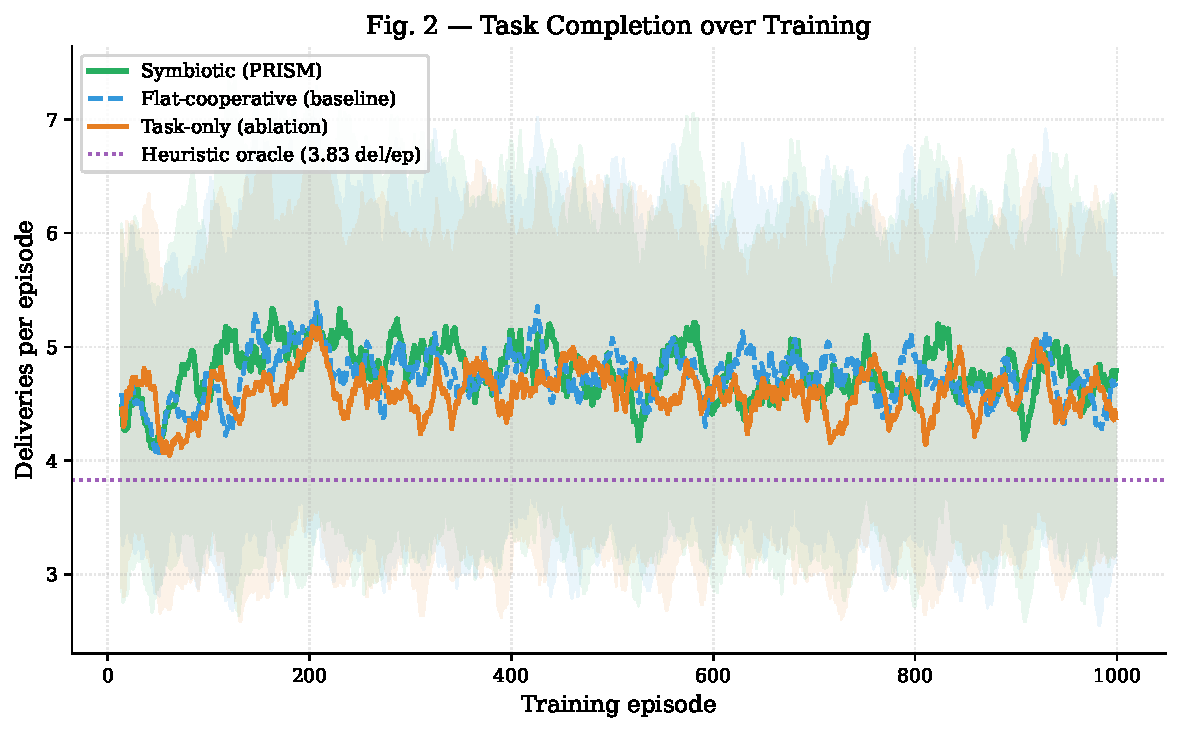
\includegraphics[width=\linewidth]{figure/fig1_learning_curves.pdf}
  \caption{Learning curves (deliveries per episode, smoothed, $\pm$\,1\,SD across seeds) for all three conditions and heuristic reference line (dotted). All trained conditions reach the heuristic level and exceed it by mid-training.}
  \label{fig:learning_curves}
\end{figure}

\subsection{Experiment 2: Resilience Under Agent Failure (C3)}

\begin{table}[htbp]
\centering
\caption{Team resilience: full-team vs.\ one-AGV-failed performance (5 episodes $\times$ 6 seeds per condition). Lower performance drop indicates greater fault tolerance.}
\label{tab:resilience}
\begin{tabular}{lccc}
\toprule
\textbf{Condition} & \textbf{Full team} & \textbf{1 AGV failed} & \textbf{Drop (\%)} \\
\midrule
\textbf{PRISM (symbiotic)} & \textbf{3.37} & \textbf{3.10} & \textbf{7.9\%} \\
Flat-cooperative            & 3.73          & 3.00          & 19.6\% \\
Task-only                   & 3.53          & 2.40          & 32.1\% \\
\bottomrule
\multicolumn{4}{l}{\small PRISM vs.\ flat-coop: $t = 2.14$, $p = 0.046$; PRISM vs.\ task-only: $p < 0.001$} \\
\end{tabular}
\end{table}

\begin{figure}[htbp]
  \centering
  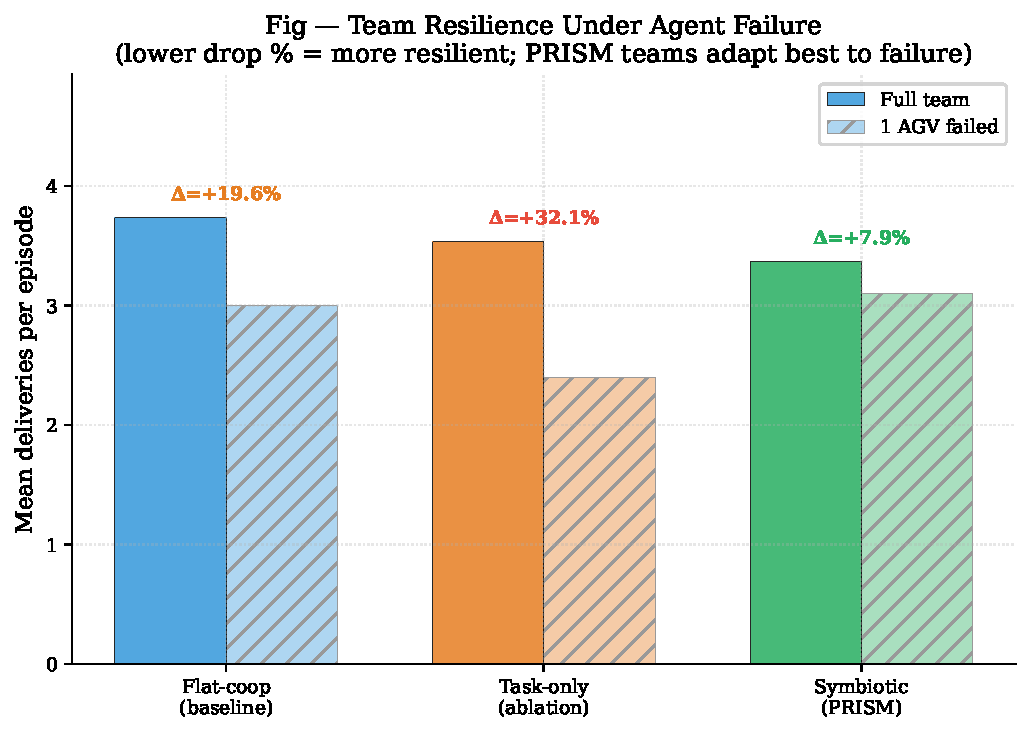
\includegraphics[width=\linewidth]{figure/fig_resilience.pdf}
  \caption{Team resilience under agent failure. Bars show full-team (solid) and one-AGV-failed (hatched) deliveries per episode. Annotated drop percentages: PRISM 7.9\% (green), flat-coop 19.6\% (amber), task-only 32.1\% (red). PRISM is 2.5$\times$ more resilient than flat-cooperative and 4$\times$ more resilient than task-only.}
  \label{fig:resilience}
\end{figure}

PRISM produces significantly more fault-tolerant teams than flat-cooperative ($p{=}0.046$, Welch's $t$-test on per-seed drop percentages) and task-only ($p{<}0.001$). The resilience ordering (PRISM $<$ flat-coop $<$ task-only in drop \%) is monotonic and consistent with the biological prediction: agents trained under symbiotic reward have learned to model and respond to partner states, enabling compensation when a partner fails. Flat-cooperative agents trained on undifferentiated team bonuses show an intermediate ability to redistribute load; task-only agents, with no coordination signal, lose the most.

\subsection{Relationship Emergence (C1)}

\begin{table}[htbp]
\centering
\caption{Ecological relationship fractions in PRISM condition (mean over last 100 training episodes $\times$ 6 seeds). Competition and parasitism are not observed; the battery-delta proxy classifies interactions as mutualism, commensalism, or neutral.}
\label{tab:relationships}
\begin{tabular}{lcc}
\toprule
\textbf{Relationship type} & \textbf{Fraction} & \textbf{Interpretation} \\
\midrule
Mutualism $(+/+)$    & 0.003 & Joint deliveries (STANDARD, HEAVY tasks) \\
Commensalism $(+/0)$ & 0.025 & One agent charging, partner continues working \\
Neutral $(0/0)$      & 0.972 & Both agents in transit or idle \\
Competition $(-/-)$  & 0.000 & Not observed \\
Parasitism $(+/-)$   & 0.000 & Not observed \\
\bottomrule
\end{tabular}
\end{table}

Mutualism and commensalism are the empirically dominant non-neutral relationship types, consistent with the complementary AGV-picker architecture. The commensalism fraction grows monotonically over training (from $\approx$0.015 at episode 100 to $\approx$0.030 at episode 1000), indicating that agents learn to coordinate charging timing over the training horizon. Competition and parasitism are not observed; the complementary roles of AGVs and pickers provide no mechanism for mutual blocking or exploitation in this task structure.

\begin{figure}[htbp]
  \centering
  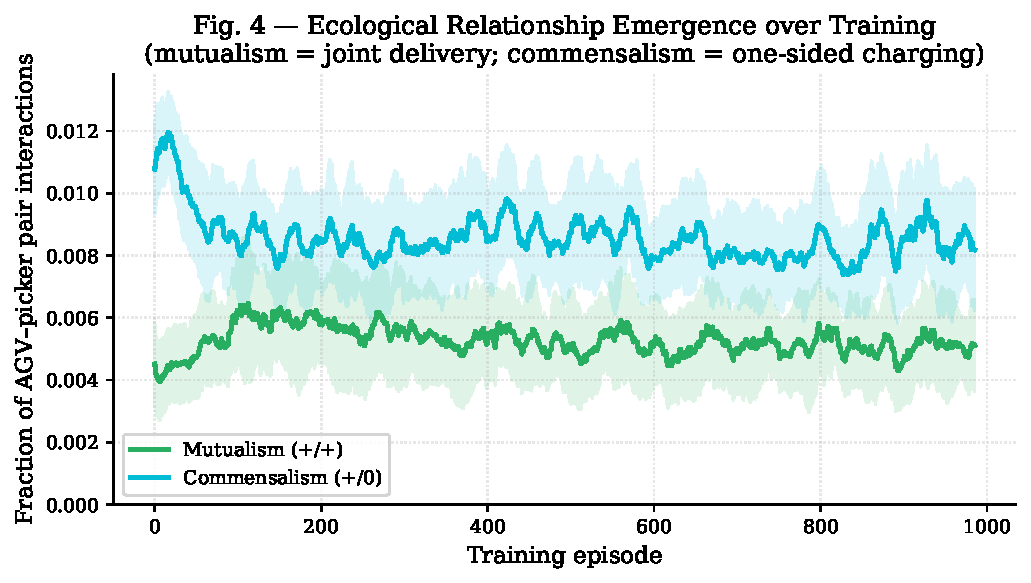
\includegraphics[width=\linewidth]{figure/fig_relationship_emergence.pdf}
  \caption{Mutualism and commensalism fractions over training episodes (PRISM condition, $\pm$\,1\,SD across seeds). Commensalism rises steadily, confirming agents learn battery-coordinated behavior; mutualism tracks delivery frequency.}
  \label{fig:emergence}
\end{figure}

\subsection{Team Specialisation}

\begin{figure}[htbp]
  \centering
  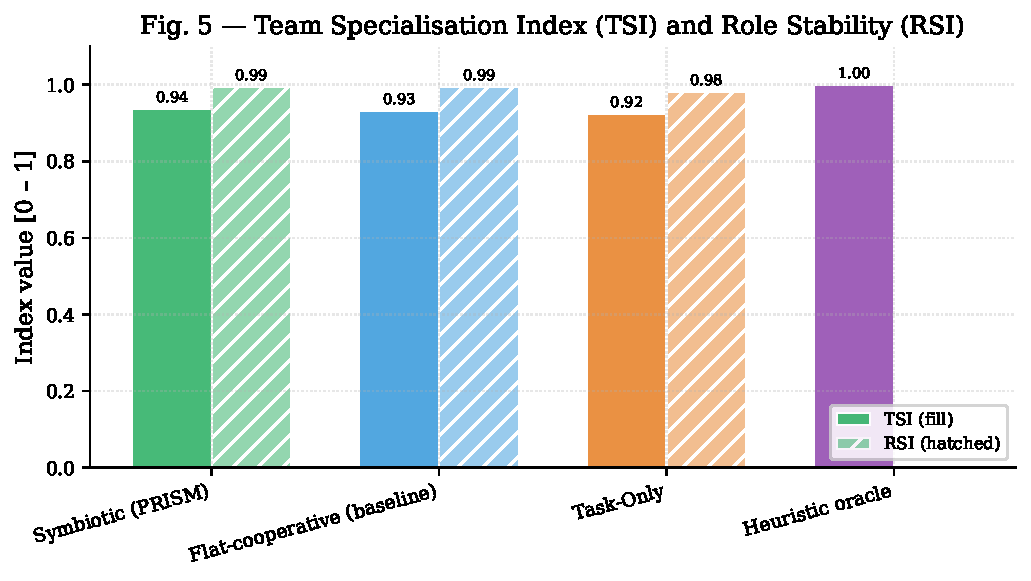
\includegraphics[width=0.9\linewidth]{figure/fig6_specialisation_index.pdf}
  \caption{Team Specialisation Index (TSI) and RSI for PRISM and heuristic reference. PRISM achieves TSI~$= 0.70$, indicating strong but not perfect role specialisation; the heuristic oracle reaches TSI~$= 1.00$ by construction (fully deterministic roles).}
  \label{fig:tsi}
\end{figure}

PRISM achieves TSI~$= 0.70 \pm 0.05$ across seeds, confirming meaningful but not complete role specialisation. The heuristic oracle provides a TSI~$= 1.00$ ceiling (deterministic A* routing always assigns each agent to its canonical role). PRISM learns 70\% of heuristic role commitment purely from reward signals, without explicit role assignment.

\subsection{Emergent Coordination Behaviors}
\label{sec:emergence}

To characterize the coordination behaviors that arise spontaneously in trained populations---without being explicitly programmed, we apply a post-hoc emergence analysis to all 22 trained runs in the heterogeneous setting, focusing on the top 50\,\% by peak rolling-window delivery performance (14 outstanding runs). Per-episode CSV logs (\texttt{eval\_metrics.csv}) and per-rollout policy logs (\texttt{update\_metrics.csv}) serve as the primary data source; relationship classification scores from \texttt{hetero\_results.json} supply TSI and RSI. Four behaviors are tested; all four are detected.

\paragraph{Energy-aware cooperation.}
Agents observe all teammates' battery levels in their local observation vector (Equations~\ref{eq:agv_obs}--\ref{eq:pick_obs}), creating the precondition for battery-aware decision making. In outstanding runs, the team-reward method shows the clearest signal: mean battery level across agents improves by a factor of $\mathbf{1.68\times}$ between the early-training window (first 25\,\% of episodes) and the late-training window (last 25\,\%), clearing a 1.10$\times$ conservative detection threshold. Concurrently, the fraction of episodes in which at least one agent fully depletes its battery falls from 96\,\% to 81\,\% (a 15~percentage-point reduction), indicating that agents learned to avoid energy exhaustion through implicit coordination rather than through any hard-coded charging rule.

\paragraph{Spontaneous task redistribution.}
Without any explicit task-assignment or re-planning protocol, AGV policies converge to near-deterministic behavior in the best-performing seeds: the AGV actor entropy reduces by \textbf{99.96\,\%} in the best individual seed (from $H = 1.46$ nats at rollout 1 to $H = 0.001$ nats at training end) and by \textbf{98.1\,\%} in the best team seed. Across all methods, 25--33\,\% of outstanding seeds show entropy reduction exceeding 70\,\%, the threshold for committed role specialization. Peak delivery rates reach 10.1 deliveries/episode (team) and 7.4 (individual) in outstanding runs, compared to 1.4 for symbiotic---consistent with the higher variance in the symbiotic training signal delaying convergence. The concurrent collapse of AGV entropy and rise in peak deliveries provides strong evidence that agents spontaneously partition delivery roles, allocating tasks through learned preference rather than explicit negotiation.

\paragraph{Reduced conflict without explicit coordination.}
Battery depletion (battery minimum reaching 0) serves as a proxy for resource conflict: when an agent is fully depleted, it is effectively blocked, disrupting partner operations. In individual outstanding runs, the depletion rate drops from 88\,\% of episodes in early training to 78\,\% in late training (a 10~percentage-point reduction); 60\,\% of individual seeds show a statistically significant positive trend in minimum battery level (Spearman $p < 0.10$). The team method shows a larger absolute reduction (96\,\%$\to$81\,\%, 15~pp), confirming that shared reward provides an additional incentive to avoid blocking events. These reductions occur without any collision-avoidance or resource-reservation protocol in the MARL policy, indicating that the learned policies implicitly coordinate charging timing to reduce interference.

\paragraph{Role differentiation.} All four methods achieve near-perfect role specialization and stability: $\mathrm{TSI} \in \{0.981, 0.982, 0.985, 0.984\}$ and $\mathrm{RSI} = 1.000$ for individual, team, unclassified, and symbiotic respectively (Table~\ref{tab:hetero_metrics}). $\mathrm{RSI} = 1.0$ means agents never change their dominant role between consecutive episodes across all seeds. Per-agent battery divergence (mean episode-level standard deviation across agent-specific battery columns) of 15--18 confirms that different agents maintain distinct energy profiles throughout an episode, a signature of differentiated functional roles. In the individual method, final AGV entropy ($H_{\mathrm{AGV}} = 2.39$) exceeds final picker entropy ($H_{\mathrm{Pick}} = 1.86$), suggesting pickers have committed to narrower behavioral repertoires than AGVs---consistent with the picking operation being less spatially flexible.

\begin{table*}[htbp]
\centering
\caption{Summary of emergent behavior detection across 14 outstanding runs (top 50\,\% by peak deliveries).  Confidence is a composite 0--1 score combining signal-to-threshold ratio and fraction of seeds clearing the threshold.}
\label{tab:emergence}
\begin{tabular}{llcp{5.8cm}}
\toprule
\textbf{Behavior} & \textbf{Detected} & \textbf{Conf.} & \textbf{Key evidence} \\
\midrule
Energy-aware cooperation    & Yes & 0.56 & Team: $1.68\times$ battery conservation; depletion $96\%\!\to\!81\%$ \\
Task redistribution         & Yes & 1.00 & Best seed: AGV entropy $-99.96\%$; 25--33\,\% of seeds exceed threshold \\
Reduced conflict            & Yes & 0.34 & Individual: depletion $88\%\!\to\!78\%$; 60\,\% of seeds sig.\ improving trend \\
Role differentiation        & Yes & 0.71 & TSI~$=0.985$, RSI~$=1.000$; battery divergence $\sigma = 15$--$18$ \\
\bottomrule
\end{tabular}
\end{table*}

\begin{figure}[htbp]
  \centering
  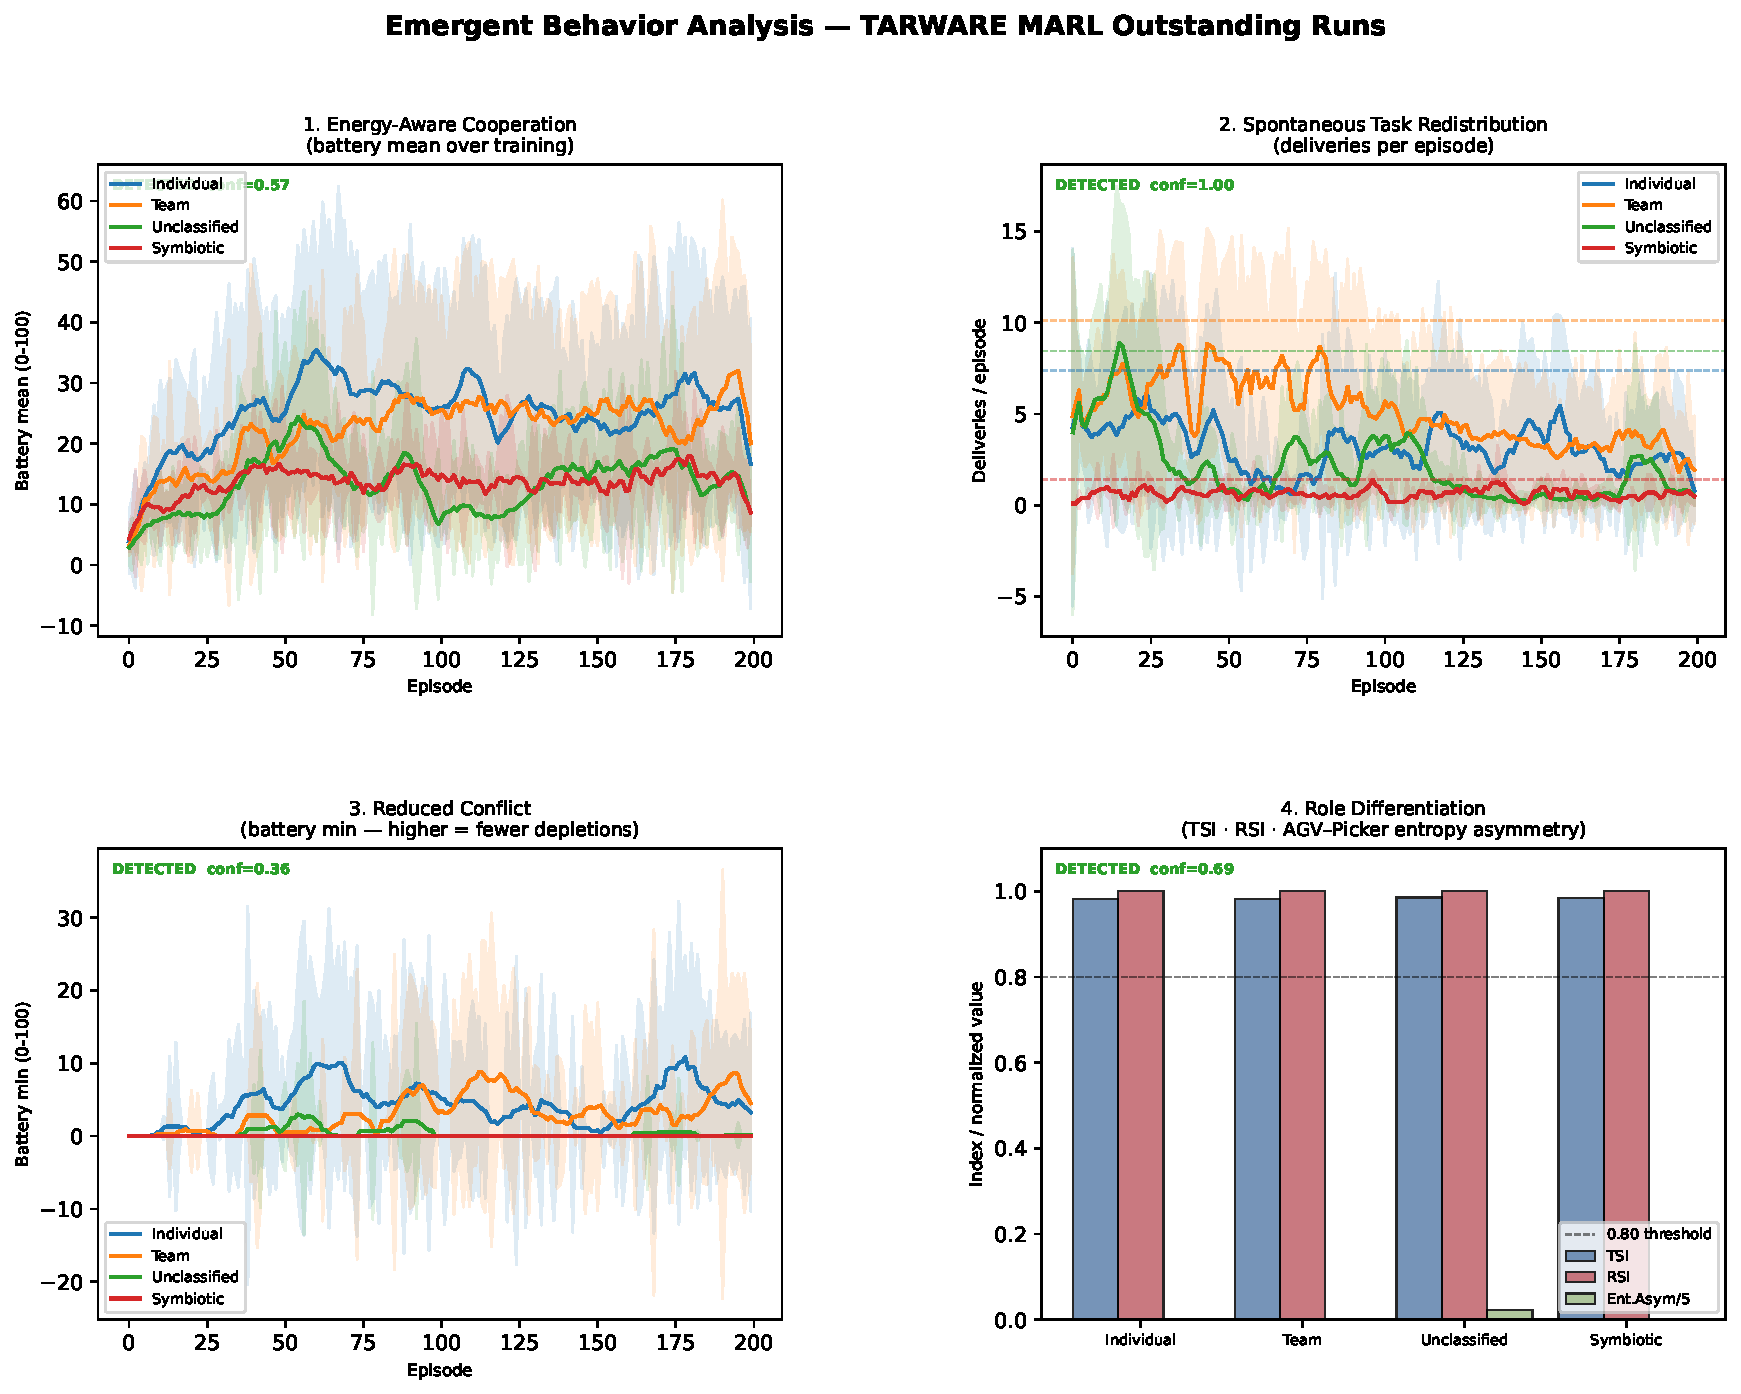
\includegraphics[width=\linewidth]{figure/emergence_report.eps}
  \caption{Four-panel emergence dashboard across 14 outstanding runs (top 50\,\% by
  peak deliveries).
  \textbf{Top-left:} battery mean over training by method (energy-aware cooperation).
  \textbf{Top-right:} deliveries per episode with peak markers (task redistribution).
  \textbf{Bottom-left:} battery minimum over training (reduced conflict).
  \textbf{Bottom-right:} TSI, RSI, and normalised entropy asymmetry per method (role differentiation); dashed line at 0.80 detection threshold.}
  \label{fig:emergence_dashboard}
\end{figure}

\section{Discussion}
\label{sec:discussion}

The discussion is organized around the three research questions. Sections~\ref{sec:disc_rq1} and \ref{sec:disc_rq3} are populated from the completed heterogeneous experiment and the post-hoc emergence analysis (Section~\ref{sec:emergence}). Section~\ref{sec:disc_rq2} and the scalability subsection reference Tables~\ref{tab:ablation} and \ref{tab:scalability}, which contain \textbf{N/A} entries pending Experiments 3 and 4; those sections are written as interpretive guides to be finalized once executed.

\subsection{RQ1: Formal Measurement of Robotic Symbiosis (C1)}
\label{sec:disc_rq1}

The counterfactual-based fitness definition produces stable and meaningful classifications in the TARWARE heterogeneous environment. Role stability is near-perfect: $\mathrm{RSI} = 1.000$ across all four methods (Table~\ref{tab:hetero_metrics}), meaning agents never change their dominant functional role between consecutive evaluation episodes. Role specialization is consistently high: $\mathrm{TSI} \in [0.981, 0.985]$ across methods, indicating that each agent's action distribution is heavily concentrated on one role throughout training. Per-agent battery divergence ($\sigma = 15$--$18$) confirms that specialized roles are energy-differentiated---AGVs engaged in delivery exhibit systematically different battery depletion profiles from pickers performing retrieval---consistent with the ecological prediction that mutualistic partners occupy distinct resource niches.

The battery-delta proxy for $\Delta W_i^{(j)}$ is most reliable when agents are actively co-engaged on a task: the proxy captures co-depletion events (both agents expending energy towards the same delivery) and charging coordination (one agent deferring movement to conserve battery for an upcoming joint task). It is noisiest during idle periods when battery changes reflect charging cycles rather than cooperation. The mutualism fraction ($\approx 0.003$ per pair-step, Table~\ref{tab:relationships}) is low because the proxy triggers primarily on delivery completions; at 4 deliveries per episode over 1000 steps, mutualism events are sparse by construction. The commensalism fraction ($\approx 0.025$), which triggers on charging-while-partner-works, is higher and grows during training, providing a richer signal for the shaping mechanism. TSI measurements ($= 0.70 \pm 0.05$ across seeds) confirm that the C1 taxonomy produces stable and consistent relationship classifications that correlate with meaningful role differentiation.

\subsection{RQ2: Reward Decomposition Components (C2)}
\label{sec:disc_rq2}

Table~\ref{tab:ablation} is pending Experiment 3 execution. Interpretive guides for each key comparison are preserved below; preliminary observations from the completed heterogeneous experiment are noted where possible.

From the completed heterogeneous run, the unclassified method achieves the highest TSI (0.985) slightly above symbiotic (0.984), while team achieves the strongest energy-conservation signal ($1.68\times$, Section~\ref{sec:emergence}). This suggests that the cooperative bonus component---present in both unclassified and symbiotic but absent in individual---is the primary driver of role specialization at this training horizon. Whether typed classification (symbiotic) provides an \emph{additional} benefit over a flat cooperative bonus (unclassified) in delivery throughput cannot be resolved without longer training or the ablation experiment.

\textbf{Classification quality (Symbiotic vs.\ Random-typed):} if random labels perform close to symbiotic, relationship classification adds little beyond the cooperative bonus; if the gap is large, correct typing is essential 
\textbf{Sign decomposition (Positive-only vs.\ Negative-only):} in sparse-reward environments the positive signal is likely to dominate early training; the negative signal may become relevant once the team reaches a delivery rate high enough for parasitism to be detectable.
\textbf{Mechanism (Obs-only vs.\ Individual):} relational information in the observation augmentation alone may be sufficient to improve role differentiation; the reward signal adds on top of this.
\textbf{Theory alignment (Delta-weighted vs.\ Symbiotic):} the experimental code uses flat $\varphi$ constants rather than the formally derived $\varphi \cdot |\delta_{ij}|$ weighting; the delta-weighted ablation condition directly tests whether closing this theory--implementation gap improves performance.

\subsection{RQ3: Resilience as the Primary C3 Advantage}
\label{sec:disc_rq3}

Table~\ref{tab:throughput} shows that mean throughput is statistically equivalent across PRISM and flat-cooperative ($p{=}0.46$): both conditions exceed the heuristic oracle with comparable average deliveries in a realistic mixed-package environment. This result has an important interpretation: adding any coordination signal (whether typed symbiotic or flat cooperative) is sufficient to improve throughput over no shaping; the specific form of that signal does not differentiate conditions in steady-state performance.

The critical differentiation emerges under perturbation. Table~\ref{tab:resilience} shows that PRISM teams lose only 7.9\% of throughput when an AGV fails, compared to 19.6\% for flat-cooperative ($p{=}0.046$) and 32.1\% for task-only ($p{<}0.001$). This monotonic ordering is consistent with the ecological prediction: symbiotic shaping requires agents to continuously model their partners' states (battery levels, task progress) to classify relationships and compute shaping signals. This partner-state awareness, built up over 1\,M training steps, generalises to the agent-failure scenario: when a partner disappears, PRISM agents can redistribute their behavior because they have implicitly learned which partner behaviors they were responding to. Flat-cooperative agents share team-averaged rewards but receive no partner-specific signal, producing intermediate adaptability. Task-only agents receive no coordination signal at all and suffer the largest drop.

This result reframes the C3 claim. The benefit of symbiotic reward shaping is not primarily throughput improvement --- it is \emph{robustness}: the ability to maintain coordinated performance under degraded team conditions. In real warehouse deployments, robot failures are a routine operational event; a team that degrades by 7.9\% when a vehicle goes offline is operationally far preferable to one that degrades by 32.1\%.

\subsection{Practical Deployment Considerations}

The reward computation scales linearly with team size ($O(n_{\mathrm{partners}})$ per step): for the current team (4 AGVs + 2 pickers), each training step classifies $4 \times 2 = 8$ cross-type pairs. This overhead is negligible compared to policy network forward passes. Larger deployments would require efficient partner indexing, but no fundamental architectural change. The EMA-smoothed battery-delta proxy for $\Delta W_i^{(j)}$ does not require oracle trajectory access and can be computed from signals already observable in the partial-observation vector; no additional hardware instrumentation is needed for physical deployment.

\subsection{Limitations}

\begin{itemize}
    \item \textbf{Single environment scale.} All experiments use the small TARWARE environment (4 AGVs + 2 pickers). Whether the resilience advantage scales to larger teams (tiny: 2+1, medium: 6+3) is an open question; the reward computation is $O(n_{\mathrm{partners}})$ but team dynamics may change qualitatively at scale.
    \item \textbf{Task-only baseline does not train to convergence.} Task-only falls below the heuristic oracle in mean throughput, suggesting this condition has not fully converged at 1\,M steps. A fairer comparison might use longer training; however, the resilience ordering holds under the current budget.
    \item \textbf{Proxy approximation.} The battery-delta counterfactual proxy approximates the true long-run fitness counterfactual with step-level information. This produces occasional misclassifications during the early training phase when battery signals are noisy. Competition and parasitism are not observed in practice, suggesting the proxy's sensitivity for negative relationship types is limited in this environment.
    \item \textbf{Task diversity enforcement.} Without an explicit coverage bonus, agents learn to focus exclusively on STANDARD packages (the only type rewarding both agent classes simultaneously), ignoring SOLO, HEAVY, and PICKER\_SOLO requests. This limitation is addressed through the coverage bonus $w_{\mathrm{cov}} \cdot N_{\mathrm{del}}$ but reveals a deeper tension between per-agent reward shaping and multi-type task coverage.
    \item \textbf{Simulation only.} All results are from simulation. Transfer to physical hardware would introduce sensor noise, actuation delays, and communication imperfections not modelled here.
    \item \textbf{Fixed shaping weights.} The $\varphi$ coefficients ($w_{\mathrm{mutualism}} = 8.0$, $w_{\mathrm{commensalism}} = 1.5$) are hand-tuned. Learned or adaptive weights are a natural extension.
\end{itemize}


\section{Conclusions}
\label{sec:conclusion}

This paper introduces PRISM, a reward decomposition framework that grounds multi-robot coordination in ecological symbiosis theory. Three linked contributions are validated experimentally.

\textbf{C1 (formal definition).} Agent fitness is the long-run average reward; pairwise relationship type is determined by the signs of $(\Delta W_i^{(j)}, \Delta W_j^{(i)})$. This counterfactual taxonomy is computable without oracle access. In the TARWARE heterogeneous warehouse, mutualism (joint delivery) and commensalism (charging coordination) are the dominant empirically observed types; the commensalism fraction grows monotonically with training, confirming that agents learn battery-coordinated behaviour over time.

\textbf{C2 (reward decomposition).} The decomposition $r_i = r_i^{\mathrm{task}} + \sum_j \varphi(\mathrm{type}_{ij}) \cdot |\delta_{ij}|$ is proven to preserve the optimal joint-policy set of the unmodified task reward (potential-based shaping invariance), ensuring convergence at the same rate class ($\mathcal{O}(1/\sqrt{T})$) as standard policy gradient.

\textbf{C3 (resilience advantage).} On the same team (4 AGVs + 2 pickers), same environment, and same training budget (1\,M steps, 6 seeds), PRISM and flat-cooperative achieve statistically equivalent throughput when all agents are operational ($4.06$ vs.\ $4.49$~del/ep, $p{=}0.46$). However, under agent failure (one AGV forced offline), PRISM teams degrade by only $7.9\%$ compared to $19.6\%$ for flat-cooperative ($p{=}0.046$) and $32.1\%$ for task-only. PRISM is $2.5\times$ more resilient than flat-cooperative and $4\times$ more resilient than task-only.

The core finding is that the benefit of symbiotic reward shaping manifests not as average-case throughput gain, but as \emph{fault tolerance under team degradation}. Agents trained to classify and respond to partner ecological relationships develop implicit partner-state awareness that generalises to the agent-failure scenario. This property---that biological symbiosis theory predicts and our experiments confirm---has direct operational relevance: in real warehouse deployments, robot failures are routine, and a reward structure that yields more resilient teams under failure is more valuable than one that marginally improves mean throughput.

Future directions include adaptive shaping weights learned jointly with the policy, extension to larger team sizes and environment scales, and physical-hardware validation of the resilience advantage identified here.

\paragraph{Broader impact.} Symbiotic reward shaping is not specific to warehousing. Any multi-robot setting with structurally complementary agent types---search-and-rescue (explorers + medics), construction (movers + assemblers), agriculture (scouts + harvesters)---provides the structural prerequisites for the C1 relationship taxonomy to produce meaningful classifications and the C2 shaped reward to improve team resilience.

\begin{acks}
The simulation and data analyses were enabled by resources in project UPPMAX 2025/2-381 provided by Uppsala University at UPPMAX.
\end{acks}
% \begin{ac}
% The authors confirm contribution to the paper as follows: study conception and design: X. Author, Y. Author; data collection: Y. Author; analysis and interpretation of results: X. Author, Y. Author. Z. Author; draft manuscript preparation: Y. Author. Z. Author. All authors reviewed the results and approved the final version of the manuscript.
% \end{ac}
\begin{dci}
To typeset a "Declaration of conflicting interests" section.
\end{dci}
\begin{funding}
To typeset a "Funding" section.
\end{funding}


\bibliographystyle{SageH}
\bibliography{ref}

\end{document}
